% weil-beginners-cg
% !TEX encoding = UTF-8 Unicode
% https://app.mediafire.com/folder/cl9fzbcpsm782
% logbook https://docs.google.com/document/d/1wntBFkuCEsOjmDI1UuVIFKEpYJAQAPdWMVaammKqPqY/edit?tab=t.0
\documentclass[12pt,letterpaper]{article}

\usepackage{etoolbox}
% 1. Define the boolean variable (defaults to false)
\newbool{scribe}
% 2. Set the boolean value (\booltrue or \boolfalse)
%\booltrue{scribe} % https://docs.google.com/document/d/1DJcZrjPx_dnQfeFpTTFppo3rdrFN6FbktpK75whE2zQ/edit?tab=t.0
\boolfalse{scribe}
\ifbool{scribe}{
    \usepackage[letterpaper,total={155mm,207mm},centering]{geometry}
}{
    \usepackage[letterpaper,top=50pt,left=60pt,right=60pt,bottom=70pt]{geometry}
}

\usepackage[T1]{fontenc}
\usepackage{amssymb,amsmath,amsthm} 
%\usepackage[letterpaper,top=50pt,left=60pt,right=60pt,bottom=70pt]{geometry} % print
%\usepackage[letterpaper,total={124mm,166mm},centering]{geometry} % SMALL3 scribe last used
\usepackage{microtype}
%\usepackage{tikz-cd}\usepackage{varwidth}
\usepackage{tikz}
\usetikzlibrary{intersections,calc}%\usepackage{tikz-cd}\usepackage{varwidth}
\usepackage{pascaltriangle}
%\usepackage{comment}
\usepackage[pdfusetitle]{hyperref}
%\usepackage{showkeys}%\usepackage{showlabels}
\usepackage{float}
\usepackage{xurl}
\usepackage{biblatex} 
\addbibresource{global-bib-file-a.bib} 
\usepackage{makeidx}
\makeindex
%\setlength\parindent{0pt}
\setlength{\parskip}{5pt} % variable
\renewcommand{\baselinestretch}{1.1} % variable
\newcommand{\C}{\mathbb{C}}
\newcommand{\F}{\mathbb{F}}
\newcommand{\G}{\mathcal{G}}
\newcommand{\N}{\mathbb{N}}
\newcommand{\Q}{\mathbb{Q}}
\newcommand{\R}{\mathbb{R}}
\newcommand{\Z}{\mathbb{Z}}
\newcommand{\Zm}[1]{\Z/#1\Z}
\newcommand{\aq}{\ensuremath{\nearrow\,\nwarrow}}
\newtheorem{thm}{Theorem}%[section] \newtheorem{cor}[thm]{Corollary}
\newtheorem{lem}[thm]{Lemma} %\newtheorem{remark}[thm]{Remark}
\newtheorem{prop}[thm]{Proposition}
\newtheorem{exer}[thm]{Exercise}
\theoremstyle{definition}
\newtheorem{defn}[thm]{Definition}
\title{Exercises in ``Number Theory for Beginners'' by A. Weil} 
\author{Pierre-Yves Gaillard} 
\date{}

\begin{document}% \tiny \scriptsize \footnotesize \small \normalsize \large \Large \LARGE \huge \Huge \Gamma \Delta \Theta \Lambda \Xi \Pi \Sigma \Phi \Psi \Omega 

\maketitle 

%\begin{center} This text is available at \url{https://shorturl.at/2PrmJ}.%%{\scriptsize This text is available at \url{https://github.com/Pierre-Yves-Gaillard/weil-beginners-exercises}.}\end{center}

\begin{center}
{\scriptsize This text is available at \url{https://github.com/Pierre-Yves-Gaillard/weil-beginners-exercises}.}
\end{center}

\tableofcontents\bigskip

%\section{Introduction} %%%

The purpose of this text is to solve the exercises in André Weil's book~\cite{weil1979} (most often referred to below as ``the book''). We have taken the liberty of changing Weil's wording here and there. In the book, Weil follows the French usage of calling a real number $x$ \emph{positive} (resp. \emph{negative}) if $x\ge0$ (resp. $x\le0$). In the present text, we follow the English usage of calling $x$ \emph{positive} if $x>0$, \emph{nonnegative} if $x\ge0$, \emph{negative} if $x<0$, and \emph{nonpositive} if $x\le0$. We also added a few digressions. We have not always tried to give the ``intended solution'', but we have tried to obey the following rule: in solving Exercise~$n.m$ (that is, Exercise~$m$ in Section~$n$), use only the results which are proved in Sections~$1$ to $n$, or stated in Exercises of $1.1$ to $n.(m-1)$, or previously proved in the present text. 

\section{Supplement to Section I}\label{SsI} %%%

The first sentence of the book is: ``We assume as known the concepts of `set' and `subset'; $\in$ means `element of'.'' In the present text, we assume as known, more generally, the basic notions of elementary set theory. We just indicate that, if $X_1, \ldots,X_n$ are sets, then we denote an $n$-\textbf{tuple} \index{tuple} $x\in X_1\times\cdots\times X_n$ by 
\begin{equation}\label{Eqtuple}
x=\langle x_1, \ldots,x_n\rangle\in X_1\times\cdots\times X_n. 
\end{equation} 
(More precisely, $\langle x_1, \ldots,x_n\rangle\in X_1\times\cdots\times X_n$ if and only if $x_i\in X_i$ for all $i$.) 

Chapter II starts with the following lemma: 

\begin{lem}\label{Ldiv}
Let $d,a$ be integers, $d>0$. Then there exists a unique largest multiple $dq$ of $d$ which is $\le a$; it can be characterized by $dq\le a<d(q+1)$, or also by $a=dq+r,0\le r<d$.
\end{lem}

The author adds: ``In that relation, $r$ is called the remainder of the division of a by $d; d$ is called the divisor, and $q$ the quotient.'' Here is the proof given in the book: 

The set of integers of the form $a-dz$ with $z\in\Z$ contains positive integers, since $z$ can be taken negative and large in absolute value (i.e. $z=-N$, with $N$ a large positive integer). Apply (6) of Section~I\footnote{(6) of Section~I says: Any non-empty set of positive integers contains a least integer.} to the set of an positive integers which can be written in that form; take its smallest element $r$, and write it as $a-dq$; this is $\ge 0$ and $<d$, since otherwise $a -d(q+1)$ would belong to the same set and would be $<r$. 

Chapter V starts with the following definition. 

\begin{defn}\label{Dgroup}
A commutative (or ``abelian'') \textbf{group} \index{group} is a set $G$, together with a binary operation between elements of $G$, satisfying the following axioms (in which the group operation is denoted by $+$):

I (Associativity). $(x+y)+z=x+(y+z)$ for all $x,y,z$ in $G$. 

II (Commutativity). $x+y=y+x$ for all $x,y$ in G. 

III If $x,y$ are in $G$, the equation $x+z=y$ has a unique solution $z$ in $G$ (written $z=y-x$). 

IV There is an element in $G$, called the neutral element (and denoted by $0$) such that $0+x=x$ for all $x$ in $G$. (Page~17.) 
\end{defn} 

The notion of isomorphism between two groups is defined in the book (page~30), but not the notion of \textbf{morphism} from one group to another. We define this notion here. 

\begin{defn}\label{Dgpmor}
A map $f:G\to H$ is a \textbf{morphism} of groups \index{morphism of groups} if it satisfies $f(1)=1$ and $f(g g')=f(g)f(g')$ for all $g, g'$ in $G$ (this implies $f(g^{-1})=f(g)^{-1}$ for all $g$ in $G$). If $f$ happens to be bijective, then its inverse $f^{-1}$ is again a morphism of groups. In this case, we say that $f$ and $f^{-1}$ are \textbf{isomorphisms} of groups. \index{isomorphism of groups} 
\end{defn}

The notion of congruence modulo~$m$ is defined on page~18: 

\begin{defn}\label{Dcong}
If $m,x,y$ are integers and $m>0, x$ and $y$ are said to be \textbf{congruent modulo}~$m$ \index{congruent modulo} if $x-y$ is a multiple of $m$; then one writes $x\equiv y \pmod m$, or more briefly $x\equiv y\ (m)$. 
\end{defn}

The main properties of this relation are spelled out after the above definition. It is observed in particular that the congruence relation is compatible with integer addition and multiplication, and that it is an equivalence relation. Only the compatibility with multiplication is proved. We reproduce this proof: Property (E) of congruence is stated as follows: 

(E) $x\equiv y,\ x'\equiv y' \pmod m$ implies $xx'\equiv yy' \pmod m$. 

Then it is written: ``As to (E), it is a consequence of the identity 
$$
xx'-yy'=x(x'-y')+(x-y)y';
$$ 
verification of all the other statements is immediate.'' Here are two other proofs of (E): 

Proof 1: We have $xy\equiv x'y \pmod m$ because $xy-x'y=(x-x')y$, and we get $x'y\equiv x'y' \pmod m$ by symmetry. 

Proof 2: We have $y=x+ma, y'=x'+ma'$ for some $a,a'$, and thus $yy'=xx'+m(ax'+a'x+maa')\equiv xx' \pmod m$. 

For completeness sake we copy here properties (A) to (F) of the relation of congruence modulo~$m$:

(A) (Reflexivity) $x\equiv x \pmod m$; 

(B) (Transitivity) $x y and y=z \pmod m$ implies $x\equiv z \pmod m$; 

(C) (Symmetry) $x\equiv y \pmod m$ implies $y\equiv x \pmod m$; 

(D) $x\equiv y, x'\equiv y' \pmod m$ implies $x\equiv\pm x', y\equiv\pm y' \pmod m$; 

(E) $x\equiv y, x'\equiv y' \pmod m$ implies $xx'\equiv yy' \pmod m$; 

(F) Let $d>0$ divide $m,x$ and $y$; then $x\equiv y \pmod m$ if and only if $\frac{x}{d}\equiv\frac{y}{d} \pmod{\frac{m}{d}}$.

From this point on, we consider Lemma~\ref{Ldiv} and Properties~(A) to (F) of congruence as proved. Theorems~\ref{Tconggpmor} and \ref{Tcongringmor} below will follow from these results. 

The following definition is given on page~19: 

\begin{defn}\label{Dclass}
A \textbf{congruence class} \index{congruence class} of integers modulo $m$ is a set consisting of all the integers which are congruent to a given one modulo $m$. 
\end{defn}

We then read: ``If $x$ is any integer, we write $(x \bmod m)$ (or simply $(x)$ if no ambiguity can occur) for the congruence class of the integers congruent to $x$ modulo $m$.'' Here we depart slightly from the book and introduce the following notation: 

\begin{defn}\label{Dpim}
We denote by $\Zm{m}$ \index{Z@$\Zm{m}$} the set of congruence classes \index{set of congruence classes} modulo~$m$, and define the map $\pi_m:\Z\to\Zm{m}$ \index{P@$\pi_m$} by the condition that $x\in\pi_m(x)$ holds for all $x\in\Z$. We say that $\pi_m$ is the \textbf{natural projection} \index{natural projection} from $\Z$ to $\Zm{m}$. 
\end{defn}

We can reformulate Theorem~V.1 of the book as: 

\begin{thm}\label{Tconggpmor}
There is a unique structure of group on $\Zm{m}$ (Definition~\ref{Dpim}) making the natural projection $\pi_m:\Z\to\Zm{m}$ a morphism of groups. This group has order $m$, and is equal, as a set, to $\{\pi_m(0), \pi_m(1), \ldots, \pi_m(m-1)\}$. 
\end{thm}

This theorem follows immediately from the properties of congruence listed above. 

Here is the definition of a ring given in the book (Section~VI p.~23):

\begin{defn}\label{Dring}
A \textbf{ring} \index{ring} is a set $R$, together with two binary operations, an addition (written $+$) and a multiplication (written $\cdot$ or $\times$) satisfying the following axioms:

I. Under addition, $R$ is a group.

II. Multiplication is associative, commutative and distributive with respect to addition: $(xy)z=x(yz), xy=yx,
x(y+z)=xy+xz$ for all $x,y,z$. (Page~23.) 
\end{defn}

This definition is followed by the comment: 

If $R$ is a ring (Definition~\ref{Dring}), then, by the distributive law 
$$
(x\cdot 0)+(xz)=x(0+z)=xz,
$$ 
so that $x\cdot 0=0$ by the additive group property. Similarly, 
$$
x\cdot(-y)=-xy.
$$ 

If there is in $R$ an element $e$ such that $ex=x$ for all $x$, this is unique; for, if $f$ is also such, then $ef=f$ and $ef=fe= e$. Such an element is called the unit element and is frequently denoted by $1_R$ or by $1$; a ring is called \textbf{unitary} if it has a unit element.\footnote{In this text, we call \emph{ring} what Weil calls \emph{unitary ring}.} (End of the comment taken from the book.) 

In the same spirit as the above comment, note that, if $a$ is an element of a ring $R$, then there is at most one element $x$ such that $ax=1$. 

\begin{defn}\label{Dunit}
In the above setting, if such an $x$ exists we say the $a$ is \textbf{invertible} or is a \textbf{unit}, \index{unit} that $x$ is the \textbf{inverse} \index{inverse} of $a$, and we write $x=a^{-1}$. 
\end{defn}

The units of $R$ form a multiplicative group. 

The definition of a morphism of rings does not appear in the book, but we find it convenient to give it here: 

\begin{defn}\label{Dringmor}
A map $f:R\to S$ between rings is a \textbf{morphism of rings} \index{morphism of rings} if it satisfies $f(0)=0, f(1)=1$, as well as $f(x+y)=f(x)+f(y)$ and $f(xy)=f(x)f(y)$ for all $x,y\in R$. If $f$ happens to be bijective, then its inverse $f^{-1}$ is again a morphism of rings. In this case, we say that $f$ and $f^{-1}$ are \textbf{isomorphisms} of rings. \index{isomorphism of rings} 
\end{defn}

Theorem~\ref{Tconggpmor} generalizes to: 

\begin{thm}\label{Tcongringmor}
There is a unique structure of ring on $\Zm{m}$ (Definition~\ref{Dpim}) making the natural projection $\pi_m:\Z\to\Zm{m}$ a morphism of rings. This ring has $m$ elements, and is equal, as a set, to $\{\pi_m(0), \pi_m(1), \ldots, \pi_m(m-1)\}$.
\end{thm}

This theorem follows immediately from the properties of congruence listed above. 

\begin{lem}\label{Luv} 
If $u,v$ are elements of a ring $R$ such that $u$ is a unit and $uv=0$, then $v=0$. 
\end{lem} 

\begin{proof} 
We have $v=u^{-1}uv=u^{-1}0=0$.
\end{proof} 

\begin{lem}\label{Lbez} 
The following conditions on the positive integers $a,b$ are equivalent: 
\begin{itemize}
  \item[\emph{(a)}] there is an integer $x$ such that $ax \equiv 1 \pmod{b}$, that is, $\pi_b(a)$ is a unit, 
  \item[\emph{(b)}] there is an integer $y$ such that $by \equiv 1 \pmod{a}$, that is, $\pi_a(b)$ is a unit, 
  \item[\emph{(c)}] there are integers $x,y$ such that $ax + by =1$. 
\end{itemize}
\end{lem} 

\begin{proof} 
It suffices to note that $ax \equiv 1 \pmod{b}$ if and only if there is an integer $y$ such that $1-ax=by$, and that $by \equiv 1 \pmod{a}$ if and only if there is an integer $x$ such that $1-by=ax$. 
\end{proof} 

If these conditions are satisfied, we say that $a$ is \textbf{prime to} $b$, \index{prime to \ldots} or that $b$ is \textbf{prime to} $a$, or that $a$ and $b$ are \textbf{relatively prime}. \index{relatively prime} If $x,y$ are integers, we say the $x$ \textbf{divides} \index{divides} $y$, and we write $x\mid y$, if $y$ is a multiple of $x$, that is, if $y\in x\Z$, where $x\Z=\{xz\mid z\in\Z\}$. Note that the set of divisors of $0$ in $\Z$ is $\Z$. An element $x$ in a ring $R$ is an element $x$ in a ring $R$ is a \textbf{zero divisor} if there is a nonzero $y$ in $R$ such that $xy=0$. So, a divisor of zero is not a zero divisor in general. 

\begin{thm}[Theorem III.2 in ~\cite{weil1979}]\label{Teucl}
If $a$ divides $bc$ and is prime to $b$, then $a$ divides $c$. 
\end{thm} 

\begin{proof} 
By assumption $\pi_a(b)$ (Definition~\ref{Dpim}) is a unit and we have $\pi_a(bc)=0$, that is, $\pi_a(b)\pi_a(c)=0$. We must show $\pi_a(c)=0$. But this follows from Lemma~\ref{Luv}. 
\end{proof} 

We insist on the fact that, from now on, we regard the statements in the present section as proved. 

\section{Section I} %%%

\begin{exer}[Exercise I.1 in~\cite{weil1979}] 
Show that the relation $(-1)\cdot(-1) = +1$ is a consequence of the distributive law.
\end{exer} 

We have 
$$
0=(-1)\cdot0 = (-1)\cdot(1+(-1)) 
$$ 
$$
= (-1)\cdot1+(-1)\cdot(-1) = -1+(-1)\cdot(-1).
$$ 

\begin{exer}[Exercise I.2 in~\cite{weil1979}] 
Prove that any integer $x>1$ has either a divisor $>1$ and $\le \sqrt{x}$ or no divisor $>1$ and $<x$ (in the latter case it is called a prime; cf.~\S~IV).
\end{exer} 

Let $1=d_1<d_2<\cdots<d_n=x, n\ge2$ be the divisors of $x$. We must show that exactly one of the two conditions below holds: 

(a) $1<d_i\le\sqrt{x}$ for some $i$, 

(b) $n=2$. 

\noindent It is clear that (a) and (b) are incompatible. So, it suffices to show that $n\ge3$ implies (a), that is, assuming $\sqrt{x}<d_2<x$, it is enough to derive a contradiction. Since $\frac{x}{d_2}$ is a divisor of $x$ satisfying $1<\frac{x}{d_2}<\sqrt{x}$, we get indeed a contradiction. 

\begin{exer}[Exercise I.3 in~\cite{weil1979}] 
Prove by induction that
\[
1^3+2^3+\cdots+n^3 = \left(\frac{n(n+1)}{2}\right)^2.
\]
\end{exer}

Set 
$$
a_n=1^3+2^3+\cdots+n^3,\quad b_n=\left(\frac{n(n+1)}{2}\right)^2.
$$ 
We show $a_n=b_n$ by induction on $n$. We have $a_0=0=b_0$. Assume $n>0$ and $a_{n-1}=b_{n-1}$. Since 
$$
b_n - b_{n-1} = \left(\frac{n(n+1)}{2}\right)^2 - \left(\frac{n(n-1)}{2}\right)^2
$$ 
$$
= n^2\cdot \frac{(n+1)^2-(n-1)^2}{4} = n^3 = a_n - a_{n-1},
$$ 
we get $b_n = b_{n-1} + n^3 = a_{n-1} + n^3 = a_n$. 

\begin{exer}[Exercise I.4 in~\cite{weil1979}] 
Prove by induction that $4^{2n+1}+3^{n+2}$ is a multiple of $13$ for $n \ge 0$.
\end{exer} 

Set $a_n=4^{2n+1}+3^{n+2}$. We have $a_0=4+9=13$. Assuming the statement holds for $n$, we get 
$$
a_{n+1} = 4^{2n+3}+3^{n+3} = 16\cdot 4^{2n+1}+3\cdot 3^{n+2}
$$ 
$$
= 13\cdot 4^{2n+1} + 3\cdot (4^{2n+1} + 3^{n+2}) = 13\cdot 4^{2n+1} + 3 a_n,
$$ 
so $a_{n+1}$ is a multiple of $13$. 

\begin{exer}[Exercise I.5 in~\cite{weil1979}] 
If one is given a balance, and $n$ weights of $1,3,3^2,\ldots$, $3^{n-1}$ lb.\ respectively, show that it is possible, by placing some weights in one pan and some in the other, to weigh out any weight of $N$ lb., with $N$ an integer $\ge 1$ and $\le \frac{1}{2}(3^n-1)$. (Hint: consider all sums of the form
\[
e_0+3e_1+3^2e_2+\cdots+3^{n-1}e_{n-1},
\]
where each $e_i$ is $0$, $+1$ or $-1$.)
\end{exer}

A weight of $N$ lb. can be weighed out if and only if it is of the form $|e_0+3e_1+3^2e_2+\cdots+3^{n-1}e_{n-1}|$, where each $e_i$ is $0$, $+1$ or $-1$. Since such an $N$ cannot exceed 
$$
1+3+3^2+\cdots+3^{n-1}=\frac{3^n-1}{2},
$$ 
there is a map 
$$
f:\{-1,0,1\}^n\to\left[-\frac{3^n-1}{2},\frac{3^n-1}{2}\right]
$$ 
defined by 
$$
f(\langle e_0,\ldots,e_{n-1}\rangle)=e_0+3e_1+3^2e_2+\cdots+3^{n-1}e_{n-1}.
$$ 
(See \eqref{Eqtuple}. If $a,b$ are integers, we denote by $[a,b]$ the set of integers $x$ such that $a\le x\le b$.) It is enough to show that 
\begin{equation}\label{Eqfs}
f\text{ is surjective.}
\end{equation}
Since the source and the target of $f$ have the same cardinality $3^n$, statement \eqref{Eqfs} reduces to 
\begin{equation}\label{Eqfi}
f\text{ is injective.}
\end{equation}
Let 
$$
d=\langle d_0,\ldots,d_{n-1}\rangle,\quad e=\langle e_0,\ldots,e_{n-1}\rangle
$$ 
be in $\{-1,0,1\}^n$, and assume $d\ne e$. We must prove $f(d)\ne f(e)$. Let $k$ be the largest $i$ such that $d_i\ne e_i$. We may assume $d_k<e_k$. Then \eqref{Eqfi} reduces to 
\begin{equation}\label{Eqless}
f(d)<f(e).
\end{equation} 
Set $c_i=e_i-d_i$. Then \eqref{Eqless} reduces in turn to 
\begin{equation}\label{Eqge1} 
c_0+3c_1+3^2c_2+\cdots+3^kc_k\ge1.
\end{equation} 
We have $1\le c_k\le 2$ and $-2\le c_i\le2$ for $0\le i\le k-1$, and thus 
$$
c_0+3c_1+\cdots+3^kc_k \ge 3^kc_k - |c_0+3c_1+\cdots+3^{k-1}c_{k-1}|
$$ 
$$
\ge 3^k - 2\, (1+3+\cdots+3^{k-1}) = 3^k - (3^k-1) = 1 > 0.
$$ 
This implies \eqref{Eqge1}, and thus \eqref{Eqfs}. 

\begin{exer}[Exercise I.6 in~\cite{weil1979}]
Show that the number of terms in any polynomial of degree $d$ in $n$ variables is at most $\frac{(n+d)!}{n!\,d!}$. (Hint: use induction on $d$, and observe that the number of terms in a homogeneous polynomial of degree $d$ in $n$ variables is the same as that of a polynomial of degree $d$ in $n-1$ variables.) 
\end{exer} 

Recall that a \textbf{monomial} in $x_1,\ldots,x_n$ is a polynomial of the form $\mu=x_1^{a_1}\cdots x_n^{a_n}$, and that its \textbf{degree} is the nonnegative integer $a_1+\cdots+a_n$. Assume that this degree is $\le d$, and set $m=d+n$ and $[m]=\{1,2,\ldots,m\}$. To the above monomial $\mu$ we attach the $n$-element subset $B=\{b_1,\ldots,b_n\}$ of $[m]$ defined by $b_i=a_1+\cdots+a_i+i$ for $i=1,\ldots,n$. Since $b_1<\cdots<b_n$ (as easily checked), we see that $B$ has indeed $n$ elements. Conversely, if $B$ is such a subset with $b_1<\cdots<b_n$, we define $a_i$ recursively by $a_1=b_1-1$ and $a_i=b_i-b_{i-1}-1$ for $i=1,2,\ldots,n$. This defines a bijection between degree $\le m-n$ monomials in $x_1,\ldots,x_n$ and $n$-element subsets of $[m]$. 

Let $\binom{m}{n}$ be the number of such subsets. It suffices to prove 
\begin{equation}\label{Eqpascal}
\binom{m}{n}=\frac{m!}{n!(m-n)!}
\end{equation} 
for $0\le n\le m$. 

We prove \eqref{Eqpascal} by induction on $m$. We first observe that \eqref{Eqpascal} is obvious for $n=0$ or $n=m$, and thus for $m=0$. Assuming that \eqref{Eqpascal} holds for $m-1$ and all $n$ with $0\le n\le m$, it is enough to show that $n,m-n\ge1$ implies 
\begin{equation}\label{EqpascalI1}
\binom{m}{n}=\binom{m-1}{n}+\binom{m-1}{n-1}
\end{equation} 
and 
\begin{equation}\label{EqpascalI2}
\frac{m!}{n!(m-n)!}=\frac{(m-1)!}{n!(m-1-n)!}+\frac{(m-1)!}{(n-1)!(m-n)!}.
\end{equation} 
Let us check \eqref{EqpascalI2}: 
$$
\frac{(m-1)!}{n!(m-1-n)!}+\frac{(m-1)!}{(n-1)!(m-n)!}
$$ 

$$
=\frac{(m-1)!}{(n-1)!(m-1-n)!}\left(\frac{1}{n}+\frac{1}{m-n}\right)
$$ 

$$
=\frac{(m-1)!}{(n-1)!(m-1-n)!}\left(\frac{m}{n(m-n)}\right)
$$ 

$$
=\frac{m!}{n!(m-n)!}.
$$ 
To prove \eqref{EqpascalI1}, note that, among all the $n$-element subsets of $[m]$, there are $\binom{m-1}{n}$ of them which do not contain $m$, and so are subsets of $[m-1]$. The other $n$-element subsets of $[m]$ are obtain by adjoining $m$ to a (unique) $(n-1)$-element subset of $[m-1]$, and there are exactly $\binom{m-1}{n-1}$ such subsets. 

The positive integer $\binom{m}{n}$ are called \textbf{binomial coefficients}. \index{binomial coefficient} It is traditional and suggesting to arrange them in a triangle, called \textbf{Pascal's triangle}. Here are two pictures: 

%\centering
\begin{center}
\pascal[binom]{6} \qquad 
\pascal{6}
\end{center} 
Row $m$ starts and ends with a one. Any other entries in Row~$m$ is the sum of the two entries immediately above it. 

Here is a variant: 

% Source - https://tex.stackexchange.com/a/32660. Posted by Ian Thompson, modified by community. See post 'Timeline' for change history. Retrieved 2026-09-02, License - CC BY-SA 3.0.
\begin{table}[htbp]
\centering
\setlength{\tabcolsep}{0pt}
\begin{tabular}{ccccccccc}
  &     &     &      & 1   &      &      &     & \\
  &     &     &      & \aq &      &      &     & \\
  &     &     & 1    &     &  1   &      &     & \\
  &     &     & \aq  &     &  \aq &      &     & \\
  &     & 1   &      & 2   &      & 1    &     & \\
  &     & \aq &      & \aq &      & \aq  &     & \\
  & 1   &     & 3    &     &  3   &      & 1   & \\
  &\aq  &     & \aq  &     &  \aq &      & \aq & \\
1 &     & 4   &      & 6   &      & 4    &     & 1
\end{tabular}
\end{table}
We start with the one up on top, which is row zero, and we compute row one, row two, \ldots, inductively by the rule: ``Entry $x$ is the sum of the $y$ such that there is an arrow from $x$ to $y$''. 

\begin{thm}[Binomial Theorem\index{Binomial Theorem}]\label{Tbt}
We have 
$$
(a+b)^n=\sum_{k=0}^n \binom{n}{k} a^k\, b^{n-k}
$$ 
if $a,b,n$ are integers with $n\ge 0$. 
\end{thm}

\begin{proof}
We have 
$$
(a_1+b_1)\cdots(a_n+b_n)=\sum_S \left(\prod_{i\in S} a_i\right) \left(\prod_{i\notin S} b_i\right),
$$ 
where $S$ runs over all the subsets of $[n]=\{1,2,\ldots,n\}$. This yields 
$$
(a+b)^n=\sum_S a^{|S|}\, b^{n-|S|},
$$ 
where $|S|$ denotes the cardinality of $S$. Then we get 
$$
(a+b)^n=\sum_{k=0}^n a^k\, b^{n-k} \sum_{|S|=k} 1 = \sum_{k=0}^n \binom{n}{k} a^k\, b^{n-k}.
$$ 
\end{proof}

\section{Section II} 

Here is a restatement the two corollaries to Theorem~II.1. 

\begin{thm}\label{Tgcd}
Let $a,b,\ldots,c$ be integers. 
\begin{enumerate}
\item There is a unique integer $d\ge0$ such that the set of all linear combinations $ax+by+\ldots+cz$ of $a,b,\ldots,c$ with integral coefficients $x,y,\ldots,z$ is the set of all multiples of $d$. 
\item There is a unique integer $e\ge0$ such that $e$ is a divisor of each one of the integers $a,b,\ldots,c$, and every common divisor of these integers is a divisor of $e$. 
\item We have $d=e$. \label{It-gcd}
\end{enumerate}
\end{thm}

\begin{defn}\label{Dgcd} 
The integer $d=e$ in Item~\ref{It-gcd} of Theorem~\ref{Tgcd} is called the \textbf{greatest common divisor} \index{greatest common divisor} (or in short the \textbf{g.c.d.}) \index{g.c.d.} of $a,b,\ldots,c$; it is denoted by $(a,b,\ldots,c)$.
\end{defn}

\begin{exer}[Exercise II.1 in~\cite{weil1979}]\label{ExII1}
Prove that $(a,b,c)=((a,b),c)=(a,(b,c))$.
\end{exer} 

Recall that $x\mid a$ means ``$x$ divides $a$'' (see sentence right before Theorem~\ref{Teucl}). Notation such as 
$$
(x\mid a)\land(x\mid b)\land\cdots\land(x\mid c)
$$ 
shall mean ``$x$ divides $a$ and $x$ divides $v$ and \ldots\ and $x$ divides $c$''. 

We shall use the following characterization of $d=(a,b,\ldots,c)$: 
$$
\text{$d\ge0$ and for all integer $x$ we have}
$$ 
$$
x\mid d\iff(x\mid a)\land(x\mid b)\land\cdots\land(x\mid c).
$$ 
Then the exercise is equivalent to the following property of the Boolean operator $\land$ (``and''): for all Boolean variables $\Gamma, \Delta, \Theta$ we have 
$$
(\Gamma \land \Delta \land \Theta) \iff ((\Gamma \land \Delta) \land \Theta) \iff (\Gamma \land (\Delta \land \Theta)).
$$ 
This property of $\land$ is one of the axioms one implicitly assumes in standard mathematics. 

\subsection{Exercises II.1 to II.5} %%%

\begin{exer}[Exercise II.3 in~\cite{weil1979}]\label{ExII3}
If $p,q,r,s$ are integers such that $ps-qr=\pm 1$, and $a,b,a',b'$ are integers such that
\begin{equation}\label{EqII3}
a'=pa+qb, \qquad b'=ra+sb,
\end{equation} 
prove that $(a,b)=(a',b')$. (Hint: solve the last two equations for $a,b$.) 
\end{exer}

The equalities in \eqref{EqII3} imply that $(a,b)$ divides $(a',b')$ (even without the condition $ps-qr=\pm 1$). So, it is enough to show that $(a',b')$ divides $(a,b)$. Set $e=ps-qr$ (so $e=\pm1$) and 
$$
p'=es,\quad q'=-eq,\quad r'=-er,\quad s'=ep,
$$ 
and check that 
$$
a=p'a'+q'b',\quad b=r'a'+s'b'.
$$ 
This implies that $(a',b')$ divides $(a,b)$. 

\begin{exer}[Exercise II.2 in~\cite{weil1979}]
Prove that, in the Fibonacci sequence $1,2,3,5,8,13$, \ldots, in which each term after the second is the sum of the two preceding ones, every two consecutive terms have a g.c.d.\ equal to $1$.
\end{exer} 

Let $f_1,f_2,\ldots$ be the Fibonacci sequence $1,2,3,5,8,13,\ldots$ Then we have 
\[
f_{n+1}=0f_n+1f_{n+1}, \qquad f_{n+2}=1f_n+1f_{n+1},
\] 
and we can conclude by Exercise~\ref{ExII3}. 

\begin{exer}[Exercise II.4 in~\cite{weil1979}]\label{ExII4}
Let $a,b$ be two integers $>0$. Put $a_0=a$, $a_1=b$; for $n\ge 1$, define $a_{n+1}$ by $a_{n-1}=a_nq_n+a_{n+1}$, $0\le a_{n+1}<a_n$, provided $a_n>0$. Prove that there exists $N\ge 1$ such that $a_{N+1}=0$, and that $a_N$ is then equal to $(a,b)$.
\end{exer} 

If we had $a_n\ne0$ for all $n$, then the $a_n$ would form a decreasing sequence of nonnegative integers. Since we have 
\[
a_n=0a_{n-1}+1a_n, \qquad a_{n+1}=1a_{n-1}-q_na_n
\] 
for $0\le n\le N$, Exercise~\ref{ExII3} implies 
$$
(a,b)=(a_0,a_1)=(a_1,a_2)=\cdots=(a_N,a_{N+1})=(a_N,0)=a_N.
$$ 

\begin{exer}[Exercise II.5 in~\cite{weil1979}]\label{ExII5}
Notations being as in Exercise II.4, prove that $a_n$ can be written in the form $ax+by$, with integral $x,y$, for all $n\ge 0$ and $\le N$.
\end{exer} 

We argue by induction on $n$, the cases $n=0$ and $n=1$ being obvious. We have 
$$ 
a_{n-2}=ax_{n-2}+by_{n-2}, \qquad a_{n-1}=ax_{n-1}+by_{n-1}
$$ 
by induction hypothesis, and we get 
$$
a_n=a_{n-2}-q_{n-1}a_{n-1}=ax_{n-2}+by_{n-2}-q_{n-1}(ax_{n-1}+by_{n-1})
$$ 
$$
=a(x_{n-2}-q_{n-1}x_{n-1})+b(y_{n-2}-q_{n-1}y_{n-1}).
$$ 

\subsection{Exercise II.6} %%%

We made a whole subsection dedicated to Exercise II.6 (Exercise \ref{ExII6} below) because we added a lot of digressions. 

\begin{exer}[Exercise II.6 in~\cite{weil1979}]\label{ExII6}
Use the procedure described in Exercises~\ref{ExII4} and \ref{ExII5} to find $(a,b)$ and to solve $ax+by=(a,b)$ in each one of the following cases: \emph{(i)} $a=56$, $b=35$; \emph{(ii)} $a=309$, $b=186$; \emph{(iii)} $a=1024$, $b=729$.
\end{exer} 

Let the notation of Exercise~\ref{ExII4} be in force. We may assume $a_0>a_1>0$. Recall that, for any rational number $x$, one writes $\lfloor x\rfloor$ for the largest integer $\le x$. Set $q_1=\lfloor\frac{a_0}{a_1}\rfloor, x_0=1, y_0=0, x_1=0, y_1=1$, and define successively the nonnegative integers 
$$
a_2,x_2,y_2,q_2; a_3,x_3,y_3,q_3;\ldots
$$ 
by 
\begin{equation}\label{Eqai}
a_i=a_{i-2}-q_{i-1} a_{i-1}
\end{equation} 
\begin{equation}\label{Eqxi}
x_i=x_{i-2}-q_{i-1} x_{i-1}
\end{equation} 
\begin{equation}\label{Eqyi}
y_i=y_{i-2}-q_{i-1} y_{i-1}
\end{equation} 
\begin{equation}\label{Eqqi}
q_i=\left\lfloor\frac{a_{i-1}}{a_i}\right\rfloor,
\end{equation} 
as long as $a_i\ne0$. When $a_{n+1}=0$, we stop. So, the integers we have defined are: 
\begin{equation}\label{Elist}
a_0,x_0,y_0; a_1,x_1,y_1,q_1; a_2,x_2,y_2,q_2; \ldots ; a_n,x_n,y_n,q_n; a_{n+1}.
\end{equation} 
We have $(a_0,a_1)=a_n$ by Exercises~\ref{ExII4}. 

\begin{defn}\label{Dbez}
This algorithm is called the \textbf{extended Euclidean algorithm}, \index{extended Euclidean algorithm} and the integers $x_n$ and $y_n$ are called the \textbf{Bézout coefficients} \index{Bézout coefficients} attached to $a_0$ and $a_1$. 
\end{defn}

\begin{thm}\label{Tbez-xy}
The Bézout coefficients $x_n$ and $y_n$ satisfy $a_0 x_n + a_1 y_n = a_n$. 
\end{thm}

\begin{proof}
We show, more generally, that we have $a_0x_i+a_1y_i=a_i$ for $0\le i\le n$. We prove the latter equality by induction on $i$. The cases $i=0$ and $i=1$ are clear. For $i>1$ we get 
$$
a_0x_i+a_1y_i=a_0(x_{i-2}-q_{i-1} x_{i-1})+a_1(y_{i-2}-q_{i-1} y_{i-1})
$$ 
$$
=a_0x_{i-2}+a_1y_{i-2}-q_{i-1}(a_0x_{i-1}+a_1y_{i-1})=a_{i-2}-q_{i-1} a_{i-1}=a_i.
$$ 
This proves the result. 
\end{proof}

Now we define $u_i,v_i$ for $1\le i\le n-1$ as follows: First we set $u_{n-1}=0, v_{n-1}=1$. Then we define successively 
$$
u_{n-2}, v_{n-2}, u_{n-3}, v_{n-3}, \ldots, u_0, v_0
$$ 
by 
%\begin{alignat*}{2} u_{i-1} &=   & v_i \\ v_{i-1} &= u_i & -q_i v_i \end{alignat*} 
\begin{equation}\label{Eqsys1}
\begin{aligned}
u_{i-1} &=   & v_i \\
v_{i-1} &= u_i & -q_i v_i 
\end{aligned}
\end{equation}
for $1\le i\le n-1$. 

\begin{thm}\label{Tbez-uv0}
The integers $u_0$ and $v_0$ satisfy $a_0 u_0 + a_1 v_0 = a_n$. 
\end{thm}

\begin{proof}
We prove, more generally, that 
\begin{equation}\label{Eqbez-uvi}
a_i u_i + a_{i+1} v_i = a_n
\end{equation} 
for $0\le i\le n-1$. We denote \eqref{Eqbez-uvi} by $(S_i)$ to stress the dependence on $i$. We have 
$$
a_{n-1} u_{n-1} + a_n v_n = a_{n-1} \cdot 0 + a_n \cdot 1 = a_n,
$$ 
so $(S_{n-1})$ is true, and it suffices to show that $(S_i)$ implies $(S_{i-1})$: 
$$
a_{i-1} u_{i-1} + a_i v_{i-1} = a_{i-1} v_i + a_i (u_i-q_i v_i) 
$$ 
$$
= a_i u_i + (a_{i-1} - q_i a_i) v_i = a_i u_i + a_{i+1} v_i.
$$ 
This proves \eqref{Eqbez-uvi}.
\end{proof}

We list below the $a_i,x_i,y_i,q_i,u_i,v_i$ obtained for each of the three sub-exercises. (The following tables were generated by the Python script \url{https://shorturl.at/0w8Jh}, written by Claude.) % https://github.com/Pierre-Yves-Gaillard/weil-beginners-exercises/blob/main/ext_euclid_7_col.py - https://shorturl.at/0w8Jh

\begin{table}[H]
    \centering
    \begin{tabular}{|r|r|r|r|r|r|r|}
    \hline
    i & a  &  x &  y & q &  u &  v \\ \hline
    0 & 56 &  1 &  0 &   &  2 & -3 \\ \hline
    1 & 35 &  0 &  1 & 1 & -1 &  2 \\ \hline
    2 & 21 &  1 & -1 & 1 &  1 & -1 \\ \hline
    3 & 14 & -1 &  2 & 1 &  0 &  1 \\ \hline
    4 &  7 &  2 & -3 & 2 &    &    \\ \hline
    \end{tabular}
\end{table}

\begin{table}[htbp]
    \centering
    \begin{tabular}{|r|r|r|r|r|r|r|}
    \hline
    i & a  &  x &  y & q &  u &  v \\ \hline
    0 & 309 & 1 & 0 &  & -3 & 5 \\ \hline
    1 & 186 & 0 & 1 & 1 & 2 & -3 \\ \hline
    2 & 123 & 1 & -1 & 1 & -1 & 2 \\ \hline
    3 & 63 & -1 & 2 & 1 & 1 & -1 \\ \hline
    4 & 60 & 2 & -3 & 1 & 0 & 1 \\ \hline
    5 & 3 & -3 & 5 & 20 &  &  \\ \hline
    \end{tabular}
\end{table}

\begin{table}[H]
    \centering
    \begin{tabular}{|r|r|r|r|r|r|r|}
    \hline
    i & a  &  x &  y & q &  u &  v \\ \hline
    0 & 1024 & 1 & 0 &  & -257 & 361 \\ \hline
    1 & 729 & 0 & 1 & 1 & 104 & -257 \\ \hline
    2 & 295 & 1 & -1 & 2 & -49 & 104 \\ \hline
    3 & 139 & -2 & 3 & 2 & 6 & -49 \\ \hline
    4 & 17 & 5 & -7 & 8 & -1 & 6 \\ \hline
    5 & 3 & -42 & 59 & 5 & 1 & -1 \\ \hline
    6 & 2 & 215 & -302 & 1 & 0 & 1 \\ \hline
    7 & 1 & -257 & 361 & 2 &  &  \\ \hline
    \end{tabular}
\end{table}

Recall that $x_n$ and $y_n$ are called the \textbf{Bézout coefficients} (Definition~\ref{Dbez}). By Theorems~\ref{Tbez-xy} and \ref{Tbez-uv0}, the Bézout coefficients satisfy 
$$
a_0 x_n + a_1 y_n = a_n = a_0 u_0 + a_1 v_0
$$ 
Since there are infinitely many couples of integers $\langle\xi,\eta\rangle$ satisfying $a_0 \xi + a_1 \eta = a_n$, it is natural to ask if we have $x_n=u_0, y_n=v_0$. The answer is Yes: 

\begin{thm}\label{Txyuv} 
We have $x_n=u_0, y_n=v_0$.  
\end{thm} 

\begin{proof}[Proof] 
Recall that the $a_i$ were defined recursively by 
$$
a_i=a_{i-2}-q_{i-1} a_{i-1}.
$$ 
To make this definition similar to that of the $u_i$ and $v_i$ in \eqref{Eqsys1} we write: 
\begin{equation}\label{Eqsys2}
\begin{aligned}
a_i &=   & a_i \\
a_{i+1} &= a_{i-1} & -q_i a_i.
\end{aligned}
\end{equation} 
In the lines below we assume that the reader is familiar with matrices, their product, the transpose operation, and knows that the transpose of a product is the product of the transposes in reverse order. We introduce the matrices: 
$$
Q_i=\begin{pmatrix} 0 & 1 \\ 1 & -q_i \end{pmatrix},\quad 
A_i=\begin{pmatrix} a_i \\ a_{i+1} \end{pmatrix}, \quad X_i=\begin{pmatrix} x_i \\ x_{i+1} \end{pmatrix},
$$ 
$$
Y_i=\begin{pmatrix} y_i \\ y_{i+1} \end{pmatrix},\quad 
W_i=\begin{pmatrix} u_i \\ w_i \end{pmatrix}.
$$ 
We get 
$$
A_i=Q_iA_{i-1},\quad X_i=Q_iX_{i-1},\quad Y_i=Q_iY_{i-1},\quad W_{i-1}=Q_iW_i
$$ 
for $1\le i\le n-1$, the last equality being also valid for $i=n$, as well as 
$$
X_0=\begin{pmatrix} 1 \\ 0 \end{pmatrix}, \quad 
Y_0=\begin{pmatrix} 0 \\ 1 \end{pmatrix}, \quad 
W_{n-1}=\begin{pmatrix} 0 \\ 1 \end{pmatrix},
$$ 
$$
\begin{pmatrix} x_{n-1} \\ x_n \end{pmatrix} = X_{n-1} = Q_{n-1} \cdots Q_1 X_0 
%
= Q_{n-1} \cdots Q_1 \begin{pmatrix} 1 \\ 0 \end{pmatrix}, 
$$ 
$$ 
\begin{pmatrix} y_{n-1} \\ y_n \end{pmatrix} = Y_{n-1} = Q_{n-1} \cdots Q_1 Y_0 
%
= Q_{n-1} \cdots Q_1 \begin{pmatrix} 0 \\ 1 \end{pmatrix}, 
$$ 
\begin{equation}\label{EqQn-1Q1}
Q_{n-1} \cdots Q_1 = \begin{pmatrix} x_{n-1} & y_{n-1} \\ x_n & x_n \end{pmatrix},
\end{equation} 
$$ 
\begin{pmatrix} u_0 \\ v_0 \end{pmatrix} = W_0 = Q_1 \cdots Q_{n-1} W_{n-1} 
%
= Q_1 \cdots Q_{n-1} \begin{pmatrix} 0 \\ 1 \end{pmatrix}, 
$$ 
\begin{equation}\label{EqQ1Qn-1}
Q_1 \cdots Q_{n-1} = \begin{pmatrix} * & * \\ u_0 & v_0 \end{pmatrix}.
\end{equation} 
Since the $Q_i$ are symmetric, $Q_{n-1} \cdots Q_1$ and $Q_1 \cdots Q_{n-1}$ are each other's transpose, Theorem~\ref{Txyuv} follows from \eqref{EqQn-1Q1} and \eqref{EqQ1Qn-1}. 
\end{proof} 

Set $a=a_0, b=a_1, d=a_n$, and let $S(a,b)$ be the set of integer solutions to $ax+by=d$, that is, the set of couples $\langle\xi,\eta\rangle$ such that $a\xi+b\eta=d$. By Theorem~\ref{Txyuv}, $\langle x_n,y_n\rangle=\langle u_0,v_0\rangle$ is such a solution, and we observed that $S(a,b)$ in infinite. So, it seems natural to ask if this particular solution can be characterized by a simple property. The positive answer is provided by the theorem below. 

\begin{thm}\label{Trankin}
Assume $a>b>2$. We have $|u_0|<\frac{b}{2d}$; moreover, $\langle u_0,v_0\rangle$ is the only $\langle\xi,\eta\rangle\in S$ with $|\xi|\le\frac{b}{2d}$. Similarly, we have $|v_0|<\frac{a}{2d}$; moreover, $\langle u_0,v_0\rangle$ is the only $\langle\xi,\eta\rangle\in S(a,b)$ with $|\eta|\le\frac{a}{2d}$. 
\end{thm} 

(See \cite{gaillard_2026_euclidean}, Lemma~3.3, for related results.) We leave the case $b=2$ to the reader as an easy exercise. 

\begin{lem}\label{Lrankin}
If $a>b>0$, then we have $|u_0|\le\frac{b}{2d}$ and $|v_0|\le\frac{a}{2d}$. 
\end{lem} 

\begin{proof}
We may assume $d=1$. Since $\langle u_i,v_i\rangle\in S(a_i,a_{i+1})$ for $0\le i<n$, it suffices to show 
\begin{equation}\label{Eqrankin}
|u_i|\le\frac{a_{i+1}}{2},\quad |v_i|\le\frac{a_i}{2}
\end{equation} 
for $0\le i<n$. Recall the equalities 
$$
a_{n-1} u_{n-1} + a_n v_n = a_{n-1} \cdot 0 + a_n \cdot 1 = a_n.
$$ 
So we have $\langle u_{n-1},v_{n-1}\rangle=\langle 0,1\rangle\in S(a_{n-1},a_n)=S(a_{n-1},1)$. We must check $|u_{n-1}|\le\frac{a_n}{2}$ and $|v_{n-1}|\le\frac{a_{n-1}}{2}$, that is, $0\le\frac{1}{2}$ and $1\le\frac{a_{n-1}}{2}$. Both inequalities are obvious. So, \eqref{Eqrankin} holds in the case $i=n-1$. It is enough to prove that the case $i$ implies the case $i-1$ for $0<i<n$. We must verify 
$$
|u_{i-1}|\le\frac{a_i}{2},\quad |v_{i-1}|\le\frac{a_{i-1}}{2}
$$ 
In view of \eqref{Eqai} and \eqref{Eqsys1}, it suffices to show 
$$
|v_i|\le\frac{a_i}{2},\quad |u_i-q_iv_i|\le\frac{a_{i+1}+q_ia_i}{2}.
$$ 
The first inequality appears in \eqref{Eqrankin}. To prove the second one, note that $|u_i-q_iv_i|\le|u_i|+q_i|v_i|\le\frac{a_{i+1}}{2}+q_i\frac{a_i}{2}$. This proves the lemma. 
\end{proof}

\begin{proof}[Proof of Theorem~\ref{Trankin}] 
We may again assume $d=1$. We have $a>b>2$ by hypothesis. We start by proving $|u_0|<\frac{b}{2}$ and $|v_0|<\frac{a}{2}$. By Lemma~\ref{Lrankin}, it is enough to exclude the four cases $u_0\ne\pm\frac{b}{2}, v_0\ne\pm\frac{a}{2}$. Assume first $u_0=\frac{b}{2}$ for the sake of contradiction. We get 
$$
1=a\cdot\frac{b}{2}+bv_0=b\left(\frac{a}{2}+v_0\right),
$$ 
and thus $2=b(a+2v_0)$, which contradicts $b>2$. The other three cases are similar. It only remains to show that 
$$
\langle u_0,v_0\rangle\ne\langle\xi,\eta\rangle\in S(a,b)
$$ 
implies $|\xi|>\frac{b}{2}$ and $|\eta|>\frac{a}{2}$. We have $\langle\xi,\eta\rangle=\langle u_0+kb,v_0-ka\rangle$ for some nonzero integer $k$. Since $-\frac{b}{2}<u_0<\frac{b}{2}$, this entails $|\xi|>\frac{b}{2}$. The proof of $|\eta|>\frac{a}{2}$ is similar. 
\end{proof} 

Recall that the $q_i$ were defined by \eqref{Eqqi}. It is clear that the algorithm also works if we round $\frac{a_{i-1}}{a_i}$ to the nearest integer, instead of rounding it to its floor. We need of course a convention for rational numbers of the form $n+\frac{1}{2}, n$ integer. We chose to round $n+\frac{1}{2}$ to $n$ if $n\ge0$, and to $n+1$ if $n<0$ (we want to minimize the absolute value of the rounding). We denote this rounding of the rational number $x$ by $R(x)$, so that $q_i$ is now defined by 
\begin{equation}\label{Eqnewqi}
q_i=R\left(\frac{a_{i-1}}{a_i}\right).
\end{equation} 

\begin{defn}\label{Dlreea}
This variant of the extended Euclidean algorithm (Definition~\ref{Dbez}) is called the \textbf{least-remainder extended Euclidean algorithm}. \index{least-remainder extended Euclidean algorithm} 
\end{defn}

Note that, when we proved $(a_0,a_1)=a_n$, Theorem~\ref{Tbez-xy}, \eqref{Eqbez-uvi}, Theorems~\ref{Tbez-uv0} and \ref{Txyuv}, we did not use \eqref{Eqqi}. We only used the fact that we have integers \eqref{Elist} and $u_i,v_i$ for $i=0,\ldots n-1$ satisfying $a_{n+1}=0$, \eqref{Eqai}, \eqref{Eqxi}, \eqref{Eqyi}, and \eqref{Eqsys1}. So, $(a_0,a_1)=a_n$, Theorem~\ref{Tbez-xy}, \eqref{Eqbez-uvi}, Theorems~\ref{Tbez-uv0} and \ref{Txyuv} hold also when the $q_i$ are defined by \eqref{Eqnewqi}. 

Here are the three tables (generated by the Python script \url{https://shorturl.at/eV2Os}, written by Claude) we get: % https://github.com/Pierre-Yves-Gaillard/weil-beginners-exercises/blob/main/ext_euclid_smart_rounding.py 

\begin{table}[H]
    \centering
    \begin{tabular}{|r|r|r|r|r|r|r|}
    \hline
    i & a  &  x &  y & q &  u &  v \\ \hline
    0 & 56 & 1 & 0 &  & 2 & -3 \\ \hline
    1 & 35 & 0 & 1 & 2 & 1 & 2 \\ \hline
    2 & -14 & 1 & -2 & -2 & 0 & 1 \\ \hline
    3 & 7 & 2 & -3 & -2 &  &  \\ \hline
    \end{tabular}
\end{table}

\begin{table}[htbp]
    \centering
    \begin{tabular}{|r|r|r|r|r|r|r|}
    \hline
    i & a  &  x &  y & q &  u &  v \\ \hline
    0 & 309 & 1 & 0 &  & 3 & -5 \\ \hline
    1 & 186 & 0 & 1 & 2 & 1 & 3 \\ \hline
    2 & -63 & 1 & -2 & -3 & 0 & 1 \\ \hline
    3 & -3 & 3 & -5 & 21 &  &  \\ \hline
    \end{tabular}
\end{table}

\begin{table}[H]
    \centering
    \begin{tabular}{|r|r|r|r|r|r|r|}
    \hline
    i & a  &  x &  y & q &  u &  v \\ \hline
    0 & 1024 & 1 & 0 &  & 257 & -361 \\ \hline
    1 & 729 & 0 & 1 & 1 & -104 & 257 \\ \hline
    2 & 295 & 1 & -1 & 2 & 49 & -104 \\ \hline
    3 & 139 & -2 & 3 & 2 & -6 & 49 \\ \hline
    4 & 17 & 5 & -7 & 8 & 1 & -6 \\ \hline
    5 & 3 & -42 & 59 & 6 & 0 & 1 \\ \hline
    6 & -1 & 257 & -361 & -3 &  &  \\ \hline
    \end{tabular}
\end{table}

In these three cases, the solution to the the Bézout coefficients (Definition~\ref{Dbez}) given by the  rounding \eqref{Eqnewqi} coincides with that given by the standard rounding $x\mapsto\lfloor x\rfloor$. In fact, this is always true: see \cite{gaillard_2026_euclidean}, Corollaries~7.1 and 7.2. Note, however, that the condition $|\frac{a_i}{a_{i-1}}|\le\frac{1}{2}$ for $2\le i\le n$ is not sufficient to ensure that the Bézout coefficients are given by the usual extended Euclidean algorithm. Consider for instance the case $\langle a_0,a_1,a_2\rangle=\langle 3,2,-1\rangle$: we get $q_1=2$ and the Bézout identity $1=2\cdot2-3\cdot1$, instead of $1=3\cdot1-2\cdot1$. For more details, we refer again the reader to \cite{gaillard_2026_euclidean}. % \cite{goodman1952euclid}

%\newpage

\begin{thm}\label{Tgz}
Given integers $a_0>a_1>1$, let $x_n$ and $y_n$ be the Bézout coefficients attached to $a_0$ and $a_1$ (Definition~\ref{Dbez}), and let $x'_{n'}$ and $y'_{n'}$ be defined by analogy using the rounding~\eqref{Eqnewqi} instead of the rounding~\eqref{Eqqi}. Then we have $n'\le n, |x'_{n'}|=|x_n|$ and $|y'_{n'}|=|y_n|$. 
\end{thm}

\begin{proof}
Let 
$$
a_0,x_0,y_0; a_1,x_1,y_1,q_1; a_2,x_2,y_2,q_2; \ldots ; a_n,x_n,y_n,q_n; a_{n+1}
$$ 
be the integers defined in \eqref{Elist}. Set $b_0=a_0, b_1=a_1$, and let $b_2, b_3, \ldots$, $b_m$ be the analogs of $a_2, a_3, \ldots, a_n$ obtained using the rounding~\eqref{Eqnewqi} instead of~\eqref{Eqqi}. If $m=n$ and $b_i=a_i$ for all $i$, there is nothing to prove. Otherwise, there is a least $k$ such that $b_k\ne a_k$ and $2\le k\le n-1$. 

Claim 1: $k$ is also the least $i$ such that $\frac{a_i}{a_{i-1}}>\frac{1}{2}$ and $2\le i\le n-1$. 

Indeed, by \eqref{Eqai} we have $a_{i-2}=q_{i-1} a_{i-1}+a_i$, and thus 
\begin{equation}\label{Eqaim2}
\frac{a_{i-2}}{a_{i-1}}=q_{i-1}+\frac{a_i}{a_{i-1}},
\end{equation} 
and \eqref{Eqqi} implies that $\frac{a_i}{a_{i-1}}$ is the fractional part of $\frac{a_{i-2}}{a_{i-1}}$. This proves the claim. 

Claim 2: $q_k=1$, and thus $a_{k+1}=a_{k-1}-a_k$. 

We have 
\[
\frac{1}{2}<\frac{a_k}{a_{k-1}}<1,\quad q_k=\left\lfloor\frac{a_{k-1}}{a_k}\right\rfloor,\quad 2>\frac{a_{k-1}}{a_k}>1,
\] 
so $q_k=1$. 

Claim 3: In the notation~\eqref{Eqnewqi} we have $R(\frac{a_{k-2}}{a_{k-1}})=q_{k-1}+1$. 

Setting $i=k$ in \eqref{Eqaim2} we get 
\[
\frac{a_{k-2}}{a_{k-1}}=q_{k-1}+\frac{a_k}{a_{k-1}},
\] 
and the claim follows from the fact that $\frac{a_k}{a_{k-1}}>\frac{1}{2}$ by definition of $k$. 

Set 
$$
a'_i=a_i \text{ for } 0\le i<k, \quad a'_k=-a_{k+1},
$$ 
$$
q'_i=q_i\text{ for } 1\le i\le k-2,\quad q'_{k-1}=q_{k-1}+1.
$$ 

Claim 4: $a'_k=a'_{k-2}-q'_{k-1}a'_{k-1}$. 

We have 
\[
a'_{k-2}-q'_{k-1}a'_{k-1}=a_{k-2}-(q_{k-1}+1)a_{k-1}
\] 
\[
=a_k-a_{k-1}=-a_{k+1}=a'_k,
\] 
the penultimate equality following from Claim~2. 

Claim 5: We have $a'_0=a_0, a'_1=a_1$, and $a'_i=a'_{i-2}-q'_{i-1}a'_{i-1}$ for $2\le i\le k$, and $q'_i=R(\frac{a'_{i-1}}{a'_i})$ for $1\le i\le k-1$. 

This follows from the previous claims. 

Define $x'_i$ for $0\le i\le k$ by $x'_0=x_0=1, x'_1=x_1=0$ and $x'_i=x'_{i-2}-q'_{i-1}x'_{i-1}$ for $2\le i\le k$. Similarly, define $y'_i$ for $0\le i\le k$ by $y'_0=x_0=1, y'_1=x_1=0$ and $y'_i=y'_{i-2}-q'_{i-1}y'_{i-1}$ for $2\le i\le k$. 

Claim 6: $x'_k=-x_{k+1}, y'_k=-y_{k+1}$. 

We have 
\[
x'_k=x'_{k-2}-q'_{k-1}x'_{k-1}=x_{k-2}-(q_{k-1}+1)x_{k-1}
\] 
\[
=x_k-x_{k-1}=-x_{k+1},
\] 
the penultimate equality following from Claim~2. The proof of $y'_k=-y_{k+1}$ is similar. 

If $k=n-1$, the result follows immediately from the above claims. 

Assume now $2\le k\le n-2$. 
\end{proof}

%\newpage

\subsection{Exercises II.7 and II.8} %%%

\begin{exer}[Exercise II.7 in~\cite{weil1979}]
If $a,b,\ldots,c,m$ are integers, and $m>0$, show that
\[
(ma,mb,\ldots,mc)=m\cdot(a,b,\ldots,c).
\]
\end{exer} 

We argue as in Exercise~\ref{ExII1}. If $x,y$ are rational numbers, we say the $x$ \textbf{divides} $y$, and we write $x\mid y$, if $y$ is an integer multiple of $x$, that is, if $y\in x\Z$, where $x\Z=\{xz\mid z\in\Z\}$. This generalizes the definitions we gave when $x,y$ are integers (see sentence right before Theorem~\ref{Teucl}). (I think this is not a standard terminology, but it is convenient to use here---and it will be used nowhere else.)

Set $d=(a,b,\ldots,c), e=(ma,mb,\ldots,mc)$. We must show $e=md$. For all integer $x$ we have: 
$$
x\mid e\iff(x\mid ma)\land(x\mid mb)\land\cdots\land(x\mid mc)
$$ 
$$
\iff(\tfrac{x}{m}\mid a)\land(\tfrac{x}{m}\mid b)\land\cdots\land(\tfrac{x}{m}\mid c)
$$ 
$$
\iff\tfrac{x}{m}\mid d
$$ 
$$
\iff x\mid md.
$$ 
Since $e,md\ge0$, this implies $e=md$. 

\begin{exer}[Exercise II.8 in~\cite{weil1979}]\label{ExII8}
Prove that every rational number can be written in one and only one way as $\frac{m}{n}$ with $(m,n)=1$ and $n>0$. 
\end{exer} 

Let $x$ be a rational number. The case $x=0$ is easy, so we assume $x\ne 0$. We have $x=\frac{a}{b}$ with $a, b$ nonzero integers. Since $\frac{a}{b}=\frac{-a}{-b}$, we may assume $b>0$. Letting $d$ be the gcd of $a$ and $b$ and setting $e=\frac{a}{d}, f=\frac{b}{d}$, we get $x=\frac{e}{f}$ with $e,f$ relatively prime. Assume 
$$
\frac{a}{b}=\frac{c}{d},\quad b,d>0,\quad a\ne0\ne c,\quad (a,b)=1=(c,d).
$$ 
We must show $a=c,b=d$. We have $ad=bc$. Then $a$ and $c$ have same sign. Moreover, $a$ divides $bc$ and is prime to $b$, so $a$ divides $c$ (see Theorem~\ref{Teucl}). Similarly, $c$ divides $a$, so $a=c$, so $b=d$. 

\section{Section III} 

\begin{exer}[Exercise III.1 in~\cite{weil1979}]\label{ExIII1} 
If $(a,b)=1$ and both $a$ and $b$ divide $c$, show that $ab$ divides $c$.
\end{exer} 

We have $c=ae$ for some $e$. Since $b$ divides $ae$ and is prime to $a$, Theorem~\ref{Teucl} implies that $b$ divides $e$, so $ab$ divides $ae=c$. 

\begin{exer}[Exercise III.2 in~\cite{weil1979}]\label{ExIII2}
If $m>1$ and $a$ is prime to $m$, show that the remainders obtained by dividing $a,2a,\ldots,(m-1)a$ by $m$ (cf.\ \S~II, Lemma) are the numbers $1,2,\ldots,m-1$, in some order.
\end{exer} 

In view of Theorem~\ref{Tcongringmor}, it suffices to show that, if $a$ is a unit (Definition~\ref{Dunit}) of a ring $R$, the map $R\setminus\{0\}\to R\setminus\{0\}, x\mapsto ax$ (Lemma~\ref{Luv}) is bijective. But this is clear because the inverse map is given by $x\mapsto a^{-1}x$. 

\begin{exer}[Exercise III.3 in~\cite{weil1979}]\label{ExIII3}
Show that, if $N$ is a positive integer, either it is a perfect square (i.e.\ of the form $n^2$, where $n$ is positive integer) or $\sqrt{N}$ is not a rational number. (Hint: use Exercise~\ref{ExII8}.) 
\end{exer} 

Assume that $\sqrt{N}$ is rational, that is, we have $\sqrt{N}=\frac{a}{b}$ with $a,b$ integers, $b>0$ and $(a,b)=1$, as in Exercise~\ref{ExII8}. It is enough to show that $N$ is a perfect square. We get $\frac{N}{1}=\frac{a^2}{b^2}$. We claim $(a^2,b^2)=1$. Corollary~1 to Theorem III.2 says that, if $c,d,e$ are integers, and if $c$ is prime both to $d$ and to $e$, it is prime to $de$. This implies first $(a,b^2)=1$, and then $(a^2,b^2)=1$. Now Exercise~\ref{ExII8} implies $N=a^2$, and $N$ is a perfect square. 

\begin{exer}[Exercise III.4 in~\cite{weil1979}]
Any integer $>1$ which is not a power of $2$ can be written as the sum of (two or more) consecutive positive integers. 
\end{exer} 

{\footnotesize (See \url{https://math.stackexchange.com/a/59162/660}.)} Let $s>1$ be an integer. We claim that the following conditions are equivalent: 
\begin{itemize}
  \item[(a)] $s$ is not a power of 2, 
  \item[(b)] there is a factorization $2s=ab$ of $2s$ with $a,b\ge2$ and $a$ and $b$ of opposite parity, 
  \item[(c)] $s$ is the sum of (two or more) consecutive positive integers.
\end{itemize}

It is enough to prove the claim. The equivalence of (a) and (b) is clear. We prove that (c) implies (b). Suppose 
$$
s=k+(k+1)+\cdots+(k+n-1)
$$ 
for some $k\ge1$ and $n\ge2$. Then
\begin{equation}\label{Eqcons}
s=nk+\sum_{i=0}^{n-1}i=nk+\frac{n(n-1)}{2}=\frac{n(n+2k-1)}{2},
\end{equation} 
and the factorization $2s=n(n+2k-1)$ does the job. We prove that (b) implies (c). Setting 
$$
m=\max(a,b),\quad n=\min(a,b),\quad k=\frac{m-n+1}{2},
$$ 
we get $m\ge3,n\ge2,k\ge1$ and $s=k+(k+1)+\cdots+(k+n-1)$ by \eqref{Eqcons}. 

Here is a numerical illustration. Set $s=15$. The factorizations of $2s=30$ satisfying our conditions are $30 = 2 \cdot 15 = 3 \cdot 10 = 5 \cdot 6$. 

For $30 = 2 \cdot 15$, we get $n=2, m=15, k=7, 15=7+8$. 

For $30 = 3 \cdot 10$, we get $n=3, m=10, k=4, 15=4+5+6$. 

For $30 = 5 \cdot 6$, we get $n=5, m=6, k=1, 15=1+2+3+4+5$. 

Here is a summary: 
\begin{table}[htbp]
    \centering
    \begin{tabular}{| l | r | l | c |}
    \hline
    $n$ & $m$ & $k$ & 15 \\ \hline
    2 & 15 & 7 & 7+8 \\ \hline
    3 & 10 & 4 & 4+5+6 \\ \hline
    5 &  6 & 1 & 1+2+3+4+5 \\ \hline
    \end{tabular}
\end{table}

Exercises~\ref{ExIII5} and \ref{ExIII6} below will be solved simultaneously. 

\begin{exer}[Exercise III.5 in~\cite{weil1979}]\label{ExIII5} 
Let $a$ and $b$ be two relatively prime positive integers and $n$ an integer $\ge ab$. Show that there are nonnegative integers $x,y$ such that $n=ax+by$. 
\end{exer} 

\begin{exer}[Exercise III.6 in~\cite{weil1979}]\label{ExIII6} 
Assume $a_1,\ldots,a_k$ be relatively prime positive integers and $n$ a positive integer. Using Exercise~\ref{ExIII5} and induction on $k$, show that, if $n$ is large enough, then there are nonnegative integers $x_1,\ldots,x_k$ such that $n=a_1x_1+\cdots+a_kx_k$. 
\end{exer} 

We prove Proposition 2.1 in Gallier's text~\cite{gallier_frobenius}, which gives a stronger result. 

\begin{prop}~\label{PG}
Let $a_1,\ldots,a_k$ be relatively prime positive integers with $a_1\le a_i$ for all $i$, and $n$ an integer 
$$
n \ge n_0=(a_1-1)(a_2+\cdots+a_k-1).
$$ 
Then there are nonnegative integers $x_1,\ldots,x_k$ such that 
$$
n=a_1x_1+\cdots+a_kx_k.
$$ 
\end{prop} 

\begin{lem}\label{L5}
Let $a_1,\ldots,a_k$ be relatively prime positive integers and $n$ an arbitrary integer. Then there are integers $x_1,\ldots,x_k$ such that $n=a_1x_1+\cdots+a_kx_k$ and $0\le x_i<a_1$ for $i\ge2$. 
\end{lem} 

\begin{proof}
There are integers $y_1,\ldots,y_k$ such that $n=a_1y_1+\cdots+a_ky_k$. For $i\ge2$ let $x_i\in\Z$ be integers satisfying $x_i \equiv y_i \pmod{a_1}$---see Definition~\ref{Dcong}---and $0\le x_i<a_1$. Theorem~\ref{Tcongringmor} implies 
$$
n \equiv a_2x_2+\cdots+a_kx_k \pmod{a_1},
$$ 
which means that $n - a_2x_2 - \cdots - a_kx_k$ is a multiple of $a_1$. Therefore, there is an integer $x_1$ such that $n - a_2x_2 - \cdots - a_kx_k = a_1x_1$, and the integers $x_1,\ldots,x_k$ do the job.
\end{proof} 

\begin{proof}[Proof of Proposition~\ref{PG}]
Let $n$ and $x_1,\ldots,x_k$ be as in Lemma~\ref{L5}. Since $x_2,\ldots,x_k$ are nonnegative, it is enough to show $x_1\ge0$ if $n\ge n_0$ (where $n_0$ is as in the statement of the proposition). We have 
\[
n = a_1x_1 + \sum_{i=2}^k a_ix_i \le a_1x_1 + \sum_{i=2}^k a_i(a_1-1) = a_1x_1 + m,
\]
with $m=(a_1-1)(a_2+\cdots+a_k)$, hence $x_1\ge\frac{n-m}{a_1}$, and we see that $\frac{n-m}{a_1}>-1$ implies $x_1\ge0$. We have
\[
\frac{n-m}{a_1}>-1\Leftrightarrow n>m-a_1\Leftrightarrow n\ge m-a_1+1=n_0,
\]
so $n\ge n_0$ implies $x_1\ge0$, as required.
\end{proof} 

\section{Section IV} 

Let $\N$ be the set of nonnegative integers and, for any set $X$ let $\N^{(X)}$ be the set of all maps $f:X\to\N$ such that $f(x)$ is nonzero for only finitely many values of $x$. Let $\Z_{>0}$ the set of positive integers and $P$ the set of rational primes. For any map $f:\Z_{>0}\to\N^{(P)}$ and any $m\in\Z_{>0}, p\in P$ set $f(m,p)=(f(m))(p)$. Theorem~IV.2 in the book implies: 

\begin{thm}\label{Tpdri}
There is a unique map $f:\Z_{>0}\to\N^{(P)}$ such that 
\begin{equation}\label{Eqpdri}
m=\prod_{p\in P}p^{f(m,p)}
\end{equation} 
for all $m\in\Z_{>0}$. This map is bijective and satisfies 
\begin{enumerate}
\item $f(1,p)=0$ for all $p$, 
\item $f(mn,p)=f(m,p)+f(n,p)$ for all $m,n\in\Z_{>0}$ and all $p\in P$, 
\item $m$ divides $n$ if and only if $f(m,p)\le f(n,p)$ for all $p$. 
\end{enumerate}
\end{thm}

This theorem will be often used in an implicit way in the sequel. Recall that $x\mid y$ means ``$x$ divides $y$'', where $x$ and $y$ are integers (see sentence right before Theorem~\ref{Teucl}), and that, for any rational number $x$, one writes $\lfloor x\rfloor$ for the largest integer $\le x$. 

\begin{exer}[Exercise IV.1 in~\cite{weil1979}]\label{ExIV1} 
Let $n$ be a positive integer and $p$ a prime number. Show that $f(n!,p)$ is given by 
$$
f(n!,p)=\sum_{i=1}^\infty\left\lfloor\frac{n}{p^i}\right\rfloor.
$$
\end{exer} 

First note that $f(n,p)$ is the number of positive integers $i$ such that $p^i$ divides $n$: 
$$
f(n,p)=\sum_{\substack{i>0 \\ p^i\mid n}} 1,
$$ 
so 
$$
f(n!,p)=\sum_{1\le k\le n} v(k) = \sum_{1\le k\le n} \sum_{\substack{i>0 \\ p^i\mid k}} 1 = \sum_{i>0} \sum_{\substack{1\le k\le n \\ p^i\mid k}} 1 = \sum_{i>0} \sum_{0<jp^i\le n} 1
$$ 
$$
= \sum_{i>0} \sum_{0<j\le np^{-i}} 1 
= \sum_{i>0} \sum_{0<j\le\lfloor np^{-i}\rfloor} 1 
= \sum_{i>0} \left\lfloor\frac{n}{p^i}\right\rfloor.
$$ 

\begin{exer}[Exercise IV.2 in~\cite{weil1979}]\label{Ex7} 
Prove that, if $a,b,\ldots,c$ are positive integer, then 
$$
\frac{(a+b+\cdots+c)!}{a!b!\cdots c!}
$$ 
is an integer. (Hint: using Exercise~\ref{ExIV1}, show that every prime occurs at least as many times in the numerator as in the denominator.) 
\end{exer} 

In view of Exercise~\ref{ExIV1} it is enough to show that we have 
$$
\lfloor x\rfloor+\lfloor y\rfloor+\cdots+\lfloor z\rfloor\le\lfloor x+y+\cdots+z\rfloor
$$ 
if $x,y,\ldots,z$ are rational numbers. But the latter inequality follows from the fact that $\lfloor x\rfloor+\lfloor y\rfloor+\cdots+\lfloor z\rfloor\le x+y+\cdots+z$. Indeed, if $n$ is integer and $u$ rational, then we have $\lfloor u\rfloor\le u$, and $n\le\lfloor u\rfloor$ is equivalent to $n\le u$. 

\begin{exer}[Exercise IV.3 in~\cite{weil1979}]
If $a,m,n$ are nonnegative integers, and $m\ne n$, show that the g.c.d. of $a^{2^m}+1$ and $a^{2^n}+1$ is 1 or 2 according as $a$ is even or odd. (Hint: use the fact that $a^{2^n}-1$ is a multiple of $a^{2^m}+1$ for $n>m$.) From this, deduce the existence of infinitely many primes. 
\end{exer} 

We may assume $n>m$. Setting $k=n-m,b=a^{2^m}$ and 
$$
c=b^{2^k-1}-b^{2^k-2}+\cdots+b-1,
$$ 
we get 
$$
a^{2^n}-1=a^{2^{m+k}}-1=b^{2^k}-1=(b+1)c=(a^{2^m}+1)c.
$$ 
So, if a positive integer $d$ divides $a^{2^m}+1$ and $a^{2^n}+1$, then $d$ divides also $a^{2^n}-1$, hence $d$ divides $a^{2^n}+1-(a^{2^n}-1)=2$, hence $d\le2$. If $a$ is even, then $a^{2^m}+1$ and $a^{2^n}+1$ are odd, and $d=1$, so the g.c.d. is 1. If $a$ is odd, then $a^{2^m}+1$ and $a^{2^n}+1$ are even, and the g.c.d. is 2. To deduce the existence of infinitely many primes, we set $a=2$. The integers $2^{2^n}+1,n=0,1,\ldots$ are larger than $1$, hence each $2^{2^n}+1$ has a prime divisor $p_n$, and by what we have just proved, the $p_n$ are distinct. 

\begin{exer}[Exercise IV.4 in~\cite{weil1979}]\label{ExIV4}
If $a=p^{\alpha}q^{\beta}\cdots r^{\gamma}$, where $p,q,\ldots,r$ are distinct primes and $\alpha,\beta,\ldots,\gamma$ are positive integers, prove that the number of distinct divisors of $a$, including $a$ and $1$, is
\[
(\alpha+1)(\beta+1)\cdots(\gamma+1)
\]
and that their sum is
\[
\frac{p^{\alpha+1}-1}{p-1}\cdot\frac{q^{\beta+1}-1}{q-1}\cdots\frac{r^{\gamma+1}-1}{r-1}.
\]
\end{exer}

The divisors of $a$ are the integers $p^u q^v \cdots r^w$ with 
$$
u, v, \ldots, w \ge 0,\quad u \le \alpha,\quad v \le \beta,\quad \ldots,\quad w \le \gamma.
$$ 
There are $(\alpha+1)(\beta+1)\cdots(\gamma+1)$ of them. Their sum is 
$$
\sum p^u q^v\cdots r^w = \left(\sum p^u\right) \left(\sum q^v\right)\cdots \left(\sum r^w\right)
$$ 
\[
=\frac{p^{\alpha+1}-1}{p-1}\cdot\frac{q^{\beta+1}-1}{q-1}\cdots\frac{r^{\gamma+1}-1}{r-1}.
\]

\begin{exer}[Exercise IV.5 in~\cite{weil1979}]
Prove that, if $D$ is the number of distinct divisors of $a$, their product is $a^{D/2}$.
\end{exer} 

We shall use the fact that, if $d$ is a divisor of $a$, then so is $\frac{a}{d}$, and $d<\sqrt{a}$ if and only if $\frac{a}{d} > \sqrt{a}$. Assume first that $a$ is not a square. Then $D$ is even. Set $n=\frac{D}{2}$, and let $d_1=1, d_2, \ldots, d_D=a$ be the divisors of $a$ listed increasing order. Then 
$$
d_1\cdots d_D = \left(d_1\frac{a}{d_1}\right)\cdots \left(d_n\frac{a}{d_n}\right)=a^n=a^{D/2}.
$$ 
If $a=b^2$ with $b>0$, then $D$ is odd. Set $n=\frac{D-1}{2}$. Then there are $n$ divisors $d_1,\ldots,d_n$ which are less than $b$, the set of all divisors of $a$ is $\{d_1, \ldots, d_n, b, \frac{b^2}{d_n}, \ldots, \frac{b^2}{d_1}\}$, and their product is $b^{2n+1}=b^D=a^{D/2}$. 

\begin{exer}[Exercise IV.6 in~\cite{weil1979}]
If $n,a,b,\ldots,c$ are integers $>1$, then the number of distinct integers of the form $a^{\alpha}b^{\beta}\cdots c^{\gamma}$ which are $\leq n$ (where $\alpha,\beta,\ldots,\gamma$ are nonnegative integers) is
\[
\leq \left(1+\frac{\log n}{\log a}\right)\left(1+\frac{\log n}{\log b}\right)\cdots\left(1+\frac{\log n}{\log c}\right).
\]
Using this fact, and the fact that 
\begin{equation}\label{Eqlog}
\lim_{n\to+\infty}\frac{(\log n)^r}{n}=0
\end{equation} 
for every $r>0$, prove that the number of primes is infinite. (Hint: assuming it to be finite, take for $a,b,\ldots,c$ all the distinct primes.) 
\end{exer} 

Let $A$ be the set of all integers of the form $a^{\alpha}b^{\beta}\cdots c^{\gamma}$ which are $\leq n$, and $B$ the set of all tuples $\langle\alpha,\beta,\ldots,\gamma\rangle$ (see \eqref{Eqtuple}) such that $a^{\alpha}b^{\beta}\cdots c^{\gamma}\leq n$, that is, 
$$
\alpha\log a+\beta\log b+\cdots+\gamma\log c\le\log n.
$$ 
If $\langle\alpha,\beta,\ldots,\gamma\rangle\in B$, then 
$$
\alpha\le\frac{\log n}{\log a},\quad\beta\le\frac{\log n}{\log b},\quad\cdots,\quad\gamma\le\frac{\log n}{\log c}.
$$ 
This implies 
$$
|A|\le|B|\le\left(1+\frac{\log n}{\log a}\right)\left(1+\frac{\log n}{\log b}\right)\cdots\left(1+\frac{\log n}{\log c}\right),
$$ 
where $|X|$ is the cardinality of $X$. In the setting of the hint, we note that $|A|=n$, and thus 
\[
n\leq\left(1+\frac{\log n}{\log a}\right)\left(1+\frac{\log n}{\log b}\right)\cdots\left(1+\frac{\log n}{\log c}\right).
\] 
The left-hand side is a polynomial $f(\log n)$ in $\log n$ with real coefficients, and we get 
$$
\frac{f(\log n)}{n}\ge1
$$ 
for all $n$, contradicting \eqref{Eqlog}. 

\begin{exer}[Exercise IV.7 in~\cite{weil1979}] 
If $(a,b)=1$ and $a^2-b^2$ is a perfect square, show that either $a+b$ and $a-b$ are perfect squares, or each is twice a perfect square. (Hint: show that the g.c.d. of $a+b$ and $a-b$ is $1$ or $2$.) 
\end{exer} 

We show that the g.c.d. of $a+b$ and $a-b$ is 1 or 2. Assume for the sake of contradiction that an odd prime $p$ divides $a+b$ and $a-b$. Then we see that $p$ divides $2a=(a+b)+(a-b)$ and $2b=(a+b)-(a-b)$, and thus that $p$ divides $a$ and $b$, contradiction. Similarly, if $4$ divides $a+b$ and $a-b$, then it divides also $2a=(a+b)+(a-b)$ and $2b=(a+b)-(a-b)$, hence $2$ divides $a$ and $b$, contradiction. 

Observation: Let $m,n$ be relatively prime positive integers. If $mn$ is a perfect square, then so are $m$ and $n$. 

Proof: Let $p$ be a prime divisor of $m$. Then $p$ occurs an even number of times in $mn$ and zero times in $n$. This implies that $p$ occurs an even number of times in $m$. We conclude that $m$ is a perfect square. By symmetry, $m$ is also a perfect square.

If $(a+b,a-b)=1$, the observation implies that $a+b$ and $a-b$ are perfect squares. 

If $(a+b,a-b)=2$, then $a$ and $b$ are odd (because $(a,b)=1$), and the observation shows that $\frac{a+b}{2}$ and $\frac{a-b}{2}$ are perfect squares. 

\section{Section V} 

\begin{exer}[Exercise V.1 in~\cite{weil1979}]
If $x_1,\ldots,x_m$ are $m$ integers, show that the sum of a suitable non-empty subset of that set is a multiple of $m$. (Hint: consider the distinct classes modulo~$m$ among those determined by $0,x_1,x_1+x_2,\ldots,x_1+x_2+\cdots+x_m$.) 
\end{exer}

Let $C_0, \ldots, C_m$ be the respective classes modulo~$m$ of $0,x_1,x_1+x_2,\ldots,x_1+x_2+\cdots+x_m$. Since there are exactly $m$ classes modulo~$m$, there are integers $i,j$ with $0\le i<j\le m$ and $C_i=C_j$, that is. 
$$
x_1+\cdots+x_i \equiv x_1+\cdots+x_i+x_{i+1}+\cdots+x_j \pmod{m},
$$ 
and thus 
$$
0 \equiv x_{i+1}+\cdots+x_j \pmod{m}.
$$ 
Since $i+1\le j$, there is at least one term in this sum. 

\begin{exer}[Exercise V.2 in~\cite{weil1979}]\label{ExV2} 
Prove that every perfect square (cf.\ Exercise~\ref{ExIII3}) is congruent to $0$, $1$ or $4$ modulo~$8$.
\end{exer}

Modulo $8$ we have $0^2 \equiv 0 \equiv 4^2, (\pm 1)^2 \equiv 1 \equiv (\pm 3)^2, (\pm 2)^2 \equiv 4$, and the result follows from Theorem~\ref{Tcongringmor}. 

\begin{exer}[Exercise V.3 in~\cite{weil1979}] 
Prove by induction that, if $n$ is a nonnegative integer, then $2^{2n+1} \equiv 9n^2-3n+2 \pmod{54}$.
\end{exer} 

Since $2^{2n+1} \equiv 9n^2-3n+2 \pmod{2}$, it is enough to verify 
\begin{equation}\label{EqV3a}
2^{2n+1} \equiv 9n^2-3n+2 \pmod{27}.
\end{equation} 
Since \eqref{EqV3a} holds for $n=0$, it suffices to show that it implies 
\begin{equation}\label{EqV3b}
2^{2(n+1)+1} \equiv 9(n+1)^2-3(n+1)+2 \pmod{27}.
\end{equation} 
We have 
$$
2^{2(n+1)+1}=4\cdot 2^{2n+1}\equiv 4(9n^2-3n+2)=36n^2-12n+8
$$ 
$$
\equiv 9n^2-12n+8 \pmod{27},
$$ 
as well as 
$$
9(n+1)^2-3(n+1)+2=9(n^2+2n+1)-3n-1
$$ 
$$
=9n^2+15n+8\equiv 9n^2-12n+8 \pmod{27}.
$$ 
This prove \eqref{EqV3b}. 

\begin{exer}[Exercise V.4 in~\cite{weil1979}]
Show that, if $x,y,z$ are integers, and $x^2+y^2=z^2$, then $xyz\equiv 0\pmod{60}$.
\end{exer}

We prove the contrapositive: if $xyz \not\equiv 0\pmod{60}$, then $x^2+y^2 \ne z^2$. So we assume $xyz \not\equiv 0\pmod{60}$. This is equivalent to: 
$$
\big[xyz \not\equiv 0 \pmod{3}\big] \text{ or } \big[xyz \not\equiv 0 \pmod{5}\big] \text{ or } \big[xyz \not\equiv 0 \pmod{4}\big].
$$ 

We shall use Theorem~\ref{Tcongringmor}. 

If $xyz \not\equiv 0 \pmod{3}$, then $x^2 \equiv y^2 \equiv z^2 \equiv 1 \pmod{3}$, hence $x^2+y^2-z^2 \equiv 2 \not\equiv 0 \pmod{3}$. 

If $xyz \not\equiv 0 \pmod{5}$, then each of $x^2, y^2$ and $z^2$ is congruent to $\pm 1$ mod $5$, hence $x^2+y^2-z^2$ is congruent to $-3, -1, 1$ or $3$ mod~$5$, hence $x^2+y^2-z^2 \not\equiv 0 \pmod{5}$. 

Assume $xyz \not\equiv 0 \pmod{4}$. If $x,y,z$ are odd, then 
$$
x^2+y^2-z^2 \equiv 1 \pmod{2}.
$$ 
Otherwise, two of our three integers $x, y, z$ are odd, and the third one is congruent to $2 \pmod{4}$. Hence the congruence classes modulo~$8$ of the numbers $x^2, y^2$ and $z^2$, taken in some order, are $1,1$ and $4$, and we conclude that $x^2+y^2-z^2 \equiv 4+1\pm1 \not\equiv 0 \pmod{8}$. 

\begin{exer}[Exercise V.5 in~\cite{weil1979}]
If $x_0,x_1,\ldots,x_n$ are integers, show that
\[
x_0+10x_1+\cdots+10^nx_n\equiv x_0+x_1+\cdots+x_n \pmod 9.
\]
\end{exer}

In view of Theorem~\ref{Tcongringmor}, this follows from the fact that $10 \equiv 1 \pmod{9}$. 

\begin{exer}[Exercise V.6 in~\cite{weil1979}]\label{ExV6}
Show that a necessary and sufficient condition for the pair of congruences $x \equiv a \pmod{m}$, $x \equiv b \pmod{n}$ to have a solution is that $a \equiv b \pmod{d}$, where $d=(m,n)$. If $d=1$, show that the solution is unique modulo~$mn$. 
\end{exer} 

The numbers $a,b,m,n,x,d$ (above) and $r,s,y$ (below) are integers, with $m,n,d\ge1$. We have: 
\begin{center}
there is an $x$ such that $x \equiv a \pmod{m}$ and $x \equiv b \pmod{n}$ \\
$\iff$ \\
there are $r,s$ such that $a+mr=b+ns$ \\ 
$\iff$ \\
there are $r,s$ such that $a-b=ns-mr$ \\ 
$\iff$ \\
$a \equiv b \pmod{d}$. 
\end{center} 
(See Definition~\ref{Dgcd}.) 

Assume $d=1$ and
$$
x\equiv y\pmod{m},\quad x\equiv y\pmod{n}.
$$ 
We must show $x\equiv y\pmod{mn}$. Since the integers $m$ and $n$ divide $x-y$, we see that $mn$ divides $x-y$, so $x\equiv y\pmod{mn}$. 

\begin{exer}[Exercise V.7 in~\cite{weil1979}]
If $n$ is an integer $>0$, show that any $n+1$ of the first $2n$ integers contain a pair $x,y$ such that $\frac{y}{x}$ is a power of $2$. (Hint: for each one of the given integers $x_0,x_1,\ldots,x_n$, call $x_i'$ the largest odd divisor of $x_i$, and show that at least two of these must be equal.)
\end{exer}

We have $x'_i \in \{1, 3, \ldots, 2n-1\}$. Since this set contains exactly $n$ elements, at least two of the $x'_i$ must coincide. 

\begin{exer}[Exercise V.8 in~\cite{weil1979}]
When $x,y$ are two integers $>0$, write $x\sim y$ if $\frac{y}{x}$ is a power of $2$, i.e.\ of the form $2^n$ with $n\in\Z$; show that this is an equivalence relation, and that $x\sim y$ if and only if the odd divisors of $x$ are the same as those of $y$.
\end{exer} 

Let $p_1=2, p_2, p_3, \ldots$ be the list of all primes (without repetition). In view of Exercise~\ref{ExII8} and Theorem~IV.2 (which says that a positive integer can be written in exactly one way as a product of primes), we see that, for any positive rational number $z$, there is a unique sequence $z_1, z_2, \ldots$ of integers (i.e. elements of $\Z$) such that $z_i=0$ for $i$ large enough, and 
\begin{equation}\label{Eqzp1}
z = p_1^{z_1} p_2^{z_2} p_3^{z_3} \cdots 
\end{equation} 
(This infinite product makes sense because only finitely many factors are not equal to $1$.) 

To solve the exercise, it is enough to show that $x\sim y$ if and only if the odd divisors of $x$ are the same as those of $y$, or even to show that $x\sim y$ if and only if, in the notation \eqref{Eqzp1}, we have $x_i = y_i$ for $i \ge 2$. Since 
$$ 
\frac{y}{x} = 2^{y_1-x_1} p_2^{y_2-x_2} p_3^{y_3-x_3} \cdots,
$$ 
we see that $z=\frac{y}{x}$ is a power of $2$, that is, by definition, $z_i = 0$ for $i \ge 2$, if and only if $x_i = y_i$ for $i \ge 2$, as required. 

\section{Section VI} %%% 

\begin{exer}[Exercise VI.1 in~\cite{weil1979}]\label{ExVI1}
If $F(X)$ is a polynomial with integral coefficients, and if $x \equiv y \pmod{m}$, show that $F(x) \equiv F(y) \pmod{m}$. 
\end{exer} 

This follows immediately from Theorem~\ref{Tcongringmor}. 

\begin{exer}[Exercise VI.2 in~\cite{weil1979}]
Solve the pair of congruences
\[
5x-7y\equiv 9\pmod{12}, \qquad 2x+3y\equiv 10\pmod{12};
\]
show that the solution is unique modulo~$12$.
\end{exer} 

All the congruences in the solution to this exercise hold modulo~$12$. We represent the system 
\[
ax-by\equiv e, \qquad cx+dy\equiv f
\] 
by the ``matrix'' 
$$ 
\begin{bmatrix}
ax & +by & \equiv & e\\
cx & +dy & \equiv & f
\end{bmatrix},
$$ 
and the notation 
$$ 
\begin{bmatrix}
ax & +by & \equiv & e\\
cx & +dy & \equiv & f
\end{bmatrix}
\sim
\begin{bmatrix}
a'x & +b'y & \equiv & e'\\
c'x & +d'y & \equiv & f'
\end{bmatrix}
$$ 
indicates that the systems are equivalent (i.e. have the same solutions). We have 
$$
\begin{bmatrix}
5x & -7y & \equiv & 12\\
2x & +3y & \equiv & 10
\end{bmatrix} 
\sim 
\begin{bmatrix}
5x & +5y & \equiv & -3\\
2x & +3y & \equiv & -2
\end{bmatrix} 
\sim 
\begin{bmatrix}
x & +y & \equiv & -3\\
2x & +3y & \equiv & -2
\end{bmatrix} 
$$ 
$$
\sim
\begin{bmatrix}
x & +y & \equiv & -3\\
  & y & \equiv & 4
\end{bmatrix} 
\sim 
\begin{bmatrix}
x &   & \equiv & 5\\
  & y & \equiv & 4
\end{bmatrix}.
$$ 
The equivalence of $5x+5y\equiv-3$ and $x+y\equiv-3$ holds because $5 \cdot 5\equiv 1$ and $5 \cdot 3 \equiv 3$. The equation $y \equiv 4$ is obtained by subtracting two times $x+y\equiv-3$ from $2x+3y\equiv-2$. The equation $x \equiv 5$ is obtained by subtracting $y\equiv4$ from $x+y\equiv-3$. Clearly, the last system has a unique solution (modulo~$12$). 

\begin{exer}[Exercise VI.3 in~\cite{weil1979}]
For all values of $a$ and $b$ modulo~$2$, solve
\[
x^2+ax+b\equiv 0\pmod 2.
\]
\end{exer}

Let $S(a,b)$ be the set of solutions of $x^2+ax+b\equiv 0\pmod 2$. We have: 
$$
S(0,0)=\{0\},\quad S(0,1)=\{1\},\quad S(1,0)=\{0,1\},\quad S(1,1)=\varnothing.
$$ 

\begin{exer}[Exercise VI.4 in~\cite{weil1979}]
Solve $x^2-3x+3\equiv 0\pmod 7$.
\end{exer}

The congruences below are modulo~$7$. We have 
$$
x^2-3x+3\equiv x^2+4x+3 \equiv (x+2)^2-4+3 \equiv (x+2)^2-1, %\equiv \equiv \equiv \equiv \equiv 
$$ 
$$
x^2-3x+3\equiv 0 \iff (x+2)^2 \equiv 1 
$$ 
$$
\iff x+2 \equiv \pm 1 \iff x \equiv -2\pm 1.
$$ 
So, the solutions are $-1$ and $-3$ (modulo~$7$). 

\begin{exer}[Exercise VI.5 in~\cite{weil1979}]
If $m>1$, show that the arithmetic mean of all positive integers prime to $m$ and $<m$ is $\frac{m}{2}$.
\end{exer}

Since the result holds for $m=2$, we may assume $m \ge 3$. Then the positive integers which are prime to $m$ and less than $m$ occur in disjoint pairs of the form $k, m-k$ (with $m-k \ne k$ because $m \ge 3$), and it suffices to observe that the arithmetic mean of each pair is $\frac{m}{2}$. 

\begin{exer}[Exercise VI.6 in~\cite{weil1979}]
If $m$ is any odd integer, prove that
\[
1^m+2^m+\cdots+(m-1)^m\equiv 0\pmod m.
\]
\end{exer} 

Setting $k=\frac{m-1}{2}$ we get 
$$
1^m+2^m+\cdots+(m-1)^m
$$ 
$$
=(1^m+2^m+\cdots+k^m)+((m-k)^m+\cdots+(m-2)^m+(m-1)^m)
$$ 
$$
= (1^m + (m-1)^m) + (2^m + (m-2)^m) + \cdots + (k^m + (m-k)^m)
$$ 
$$
\equiv (1^m + (-1)^m) + (2^m + (-2)^m) + \cdots + (k^m + (-k)^m)
$$ 
$$
= (1 + (-1)) + (2^m + (-2^m)) + \cdots + (k^m + (-k^m)) = 0,
$$ 
where the congruence is taken modulo~$m$. 

\begin{exer}[Exercise VI.7 in~\cite{weil1979}]
If $m,n$ are integers $>0$, and $(m,n)=1$, prove that $\varphi(mn)=\varphi(m)\varphi(n)$. (Hint: use Exercise~\ref{ExV6}.) 
\end{exer}

By Exercise~\ref{ExV6}, for all couple of integers $\langle a,b\rangle$ (see \eqref{Eqtuple}) there is an integer $x$ such that $x \equiv a \pmod{m}$ and $x \equiv b \pmod{n}$. Moreover, $x$ is unique modulo~$mn$. 

So, it is enough to show that, in the above setting, we have 
$$
(x,mn)=1 \iff (a,m)=1=(b,n),
$$ 
or, equivalently 
$$
(x,mn)>1 \iff [(a,m)>1 \text{ or }(b,n)>1].
$$ 
Let a prime $p$ divide $x$ and $mn$. We may assume $p$ divides $m$, hence $p$ divides $a$ and $m$. Conversely, if $p$ divides $a$ and $m$, then $p$ divides $x$ and $mn$. 

\begin{exer}[Exercise VI.8 in~\cite{weil1979}]
Show that, if $m>1$ and $p,q,\ldots,r$ are all the distinct prime divisors of $m$, then
\[
\varphi(m)=m\left(1-\frac{1}{p}\right)\left(1-\frac{1}{q}\right)\cdots\left(1-\frac{1}{r}\right).
\]
\end{exer}

By the previous exercise, it suffices to show $\varphi(p^n)=p^n(1-\frac{1}{p})$, that is, $\varphi(p^n)=p^n-p^{n-1}$ (where $p$ is prime and $n$ a positive integer). This is equivalent to the statement that there are exactly $p^{n-1}$ positive integers which are $\le p^n$ and not prime to $p^n$. Clearly, these integers are the positive multiples of $p$ which are $\le p^n$, that is, the $p^{n-1}$ numbers $p, 2p, 3p, \ldots, p^{n-1}\cdot p$. 

\begin{exer}[Exercise VI.9 in~\cite{weil1979}]
If $p$ is any prime, prove by induction on $n$, using the binomial formula (Theorem~\ref{Tbt}), that $n^p\equiv n\pmod p$ for all integers $n$.
\end{exer}

We prove $n^p\equiv n\pmod p$ by induction on $n \ge 0$. Since the case $n=0$ is obvious, it is enough to show that the case $n$ implies the case $n+1$. We have $(n+1)^p \equiv n^p + 1 \pmod p$ because the binomial coefficient (see~\eqref{Eqpascal})  
$$
\binom{p}{k}=\frac{p!}{k!(p-k)!}
$$ 
is divisible by $p$ for $1\le k\le p-1$ (see \eqref{Eqpascal} and Theorem~\ref{Tbt}). So 
$$
(n+1)^p \equiv n^p + 1 \equiv n+1 \pmod p.
$$ 

\begin{exer}[Exercise VI.10 in~\cite{weil1979}]\label{ExVI10} 
If $p$ is any prime, and $n\ge 0$, prove by induction on $n$ that, if $a\equiv b\pmod p$, then 
$$
a^{p^n}\equiv b^{p^n}\pmod{p^{n+1}}.
$$
\end{exer}

Since the case $n=0$ is obvious, it is enough to show that the case $n$ implies the case $n+1$. We have $b=a+pc$ for some integer $c$, and \eqref{Eqpascal}, coupled with Theorem~\ref{Tbt}, entail 
$$
b^{p^{n+1}} = (a+pc)^{p^{n+1}} = ((a+pc)^{p^n})^p = (a^{p^n} + p^{n+1} d)^p
$$ 
$$
=a^{p^{n+1}}+\sum_{k=1}^p \binom{p}{k} (a^{p^n})^{n-k}\ (p^{n+1} d)^k
$$ 
$$
=a^{p^{n+1}}+\sum_{k=1}^p \binom{p}{k} (a^{p^n})^{n-k}\ p^{(n+1)k}\ d^k
$$ 
$$
=a^{p^{n+1}}+p\ (a^{p^n})^{n-1}\ p^{n+1}\ d+\sum_{k=2}^p \binom{p}{k} (a^{p^n})^{n-k}\ p^{(n+1)k}\ d^k
$$ 
$$
\equiv a^{p^{n+1}} \pmod{p^{n+2}}
$$ 
for some integer $d$. 

\begin{exer}[Exercise VI.11 in~\cite{weil1979}]\label{ExVI11}
If $p$ is an odd prime, and 
$$
x^2\equiv y^2\pmod p,
$$ 
show that $x$ is congruent either to $y$ or to $-y$ modulo~$p$, but not to both unless $p$ divides $x$ and $y$; hence conclude that $x^2\equiv a\pmod p$ has a solution $x$ for exactly half of the integers $a$ among $1,2,\ldots,p-1$.
\end{exer}

We let $G=\F_p\setminus\{0\}$ be the group of units (Definition~\ref{Dunit}) of the field $\F_p$, and observe: 

(a) For $x\in G$ we have $-x\ne x$ (because $2\ne0$ in $\F_p$, since $p$ is an odd prime). 

(b) For $x,y\in G$ we have $x^2=y^2$ if and only if $(x-y)(x+y)=0$ if and only if $y$ is equal to $x$ or to $-x$. 

(c) For $a\in G$ the equation $x^2=a^2$ has exactly two solutions in $G$, namely $x=a$ and $x=-a$. 

(d) If $n=\frac{p-1}{2}$, then there are elements $x_1,\ldots, x_n\in G$ such that 
$$
G=\{x_1,\ldots, x_n,-x_1,\ldots,-x_n\},
$$ 
and the distinct squares in $G$ are $x_1^2,\ldots, x_n^2$. 

Indeed, (a) and (b) are clear and imply successively (c) and (d). The statement in the exercise follows from (b) and (d). 

\begin{exer}[Exercise VI.12 in~\cite{weil1979}]\label{ExVI12}
Show that the numbers of the form $x+y\sqrt{2}$, where $x$ and $y$ are integers, make up a ring; if $x,y$ range over all rational numbers, show that they make up a field.
\end{exer} 

Since 
$$
(x+y\sqrt{2})+(u+v\sqrt{2})=(x+u)+(y+v)\sqrt{2},
$$ 
$$
(x+y\sqrt{2})(u+v\sqrt{2})=(xu+2yv)+(xv+yu)\sqrt{2},
$$ 
the numbers of the form $x+y\sqrt{2}$, where $x$ and $y$ are integers, make up a ring. 

To show that, if $x,y$ range over all rational numbers, then the $x+y\sqrt{2}$ make up a field, it suffices, in view of the above equalities, to show that, if $x,y$ are rational numbers, with $x\ne0$ or $y\ne0$, then there are rational numbers $u, v$ such that 
$$
\frac{1}{x+y\sqrt{2}}=u+v\sqrt{2}.
$$ 
We first show that $x\ne0$ or $y\ne0$ implies $x+y\sqrt{2}\ne0$. Indeed, $x+y\sqrt{2}=0$ (with $x\ne0$ or $y\ne0$) would imply that $\sqrt{2}$ is rational, which it is not (Exercise~\ref{ExIII3}). Finally we note that
$$
\frac{1}{x+y\sqrt{2}}=\frac{x-y\sqrt{2}}{(x+y\sqrt{2})(x-y\sqrt{2})}=\frac{x-y\sqrt{2}}{x^2-2y^2}
$$ 
$$
=\frac{x}{x^2-2y^2}+\frac{-y}{x^2-2y^2}\ \sqrt{2}.
$$ 

\section{Section VII} %%% 

\subsection{Preliminaries} %%% 

Since some of the exercises in this section consist in proving some standard statements which are found in many textbooks, it is particularly important to know precisely what has been proved in the book so far. Recall that we have regard the statements in the Supplement to Section I (Section~\ref{SsI} above) as proved. In the present subsection we remind the reader of some other important statements which have been proved in the book up to this point. To this end, we copy below some excerpts (with minor modifications) from the book. We also add a few comments here and there. 

The definition of a group and of a subgroup makes it clear that the intersection of subgroups of a group $G$ (in any number, finite or not) is again a subgroup of $G$.

\begin{defn}\label{Dgen}
Let $a,b,\ldots,c$ be elements of a group $G$. Then the intersection $G'$ of all the subgroups of $G$ (including $G$ itself) which contain $a,b,\ldots,c$ is said to be \textbf{generated by} $a,b,\ldots,c$, \index{subgroup generated by a subset} and these are said to be \textbf{generators} \index{generators} of $G'$. This can also be expressed by saying that $G'$ is the smallest subgroup of $G$ containing $a,b,\ldots,c$; it may happen that it is no other than $G$ itself. 
\end{defn}

Let $G$ be a group, $x$ an element of $G$, and call $G_x$ the subgroup \textbf{generated by} $x$. \index{subgroup generated by a single element} Suppose that $G$ is written additively. As usual, write $-x$ for $0-x$; this must be in $G_x$. Also, write $0\cdot x$ for $0$; for every integer $n>0$, write $nx$ for the sum $x+x+\cdots+x$ of $n$ terms all equal to $x$, and $(-n)x$ for $-(nx)$; by induction on $n$, all these must be in $G_x$. Also by induction, one verifies at once the formulas 
$$
mx+nx=(m+n)x,\quad m(nx)=(mn)x
$$
for all $m,n$ in $\Z$. (Page~29.) 

For further reference, we write: 
\begin{equation}\label{Eqnx}
nx=\sum_{i=1}^n x.
\end{equation}

If $R$ is a ring (Definition~\ref{Dring}), then, by the distributive law 
$$
(x\cdot 0)+(xz)=x(0+z)=xz,
$$ 
so that $x\cdot 0=0$ by the additive group property. Similarly, 
$$
x\cdot(-y)=-xy.
$$ 

If there is in $R$ an element $e$ such that $ex=x$ for all $x$, this is unique; for, if $f$ is also such, then $ef=f$ and $ef = fe = e$. Such an element is called the unit element and is frequently denoted by $1_R$ or by $1$; a ring is called \textbf{unitary} if it has a unit element.\footnote{In this text, we call \emph{ring} what Weil calls \emph{unitary ring}.}

\begin{thm}[Theorem VI.3 in~\cite{weil1979}]\label{TVI3b}
For any integer $m>1$, the ring $\Zm{m}$ of congruence classes modulo~$m$ is a field if and only if $m$ is a prime. 
\end{thm}

\begin{proof} 
If $m$ is a prime, all classes modulo~$m$, other than $0$, are prime to $m$ and therefore make up a multiplicative group, by the corollary of Theorem~VI.2. On the other hand, if $m$ is not a prime, it has a divisor $d$ which is $>1$ and $<m$; then $1<d<m$, so that the congruence classes $\pi_m(d)$ and $\pi_m(\frac{m}{d})$ (Definition~\ref{Dpim}) are not $0$ while their product is $0$. Therefore they are nonzero zero-divisors, and the ring $\Zm{m}$ is not a field. 
\end{proof} 

If $p$ is a prime, the field $\Zm{p}$ of congruence classes modulo~$p$ will be denoted by $\F_p$; it has $p$ elements. 

\begin{thm}[Theorem VII.2 in ~\cite{weil1979}]\label{TVII2a}
Let $G$ be a group under addition, generated by a single element $x$. Then either $G$ is infinite, and the mapping $ax \mapsto a$ is an isomorphism (see Definition~\ref{Dgpmor}) of $G$ onto the additive group $\Z$, or it consists of a finite number $m$ of elements, and then the mapping $ax \mapsto \pi_m(a)$ (Definition~\ref{Dpim}) is an isomorphism of $G$ onto the additive group $\Zm{m}$ of congruence classes modulo~$m$ in $\Z$. 
\end{thm}

(In the book, the group $G$ in the above theorem is written multiplicatively.) Here is a reformulation of Theorem~\ref{TVII2a}: 

\begin{thm}\label{TVII2b}
Let $G$ be a group under addition and $x$ an element of $G$. Then there is a unique morphism of groups $f:\Z\to G$ such that $f(1)=x$. This morphism is given by $n\mapsto nx$ (see \eqref{Eqnx}). The image $f(\Z)$ of $Z$ under $f$ is the subgroup $H$ of $g$ generated by $x$. Either $H$ is infinite, and $f$ induces an isomorphism $\Z\simeq H$, or $H$ consists of a finite number $m$ of elements, and then the mapping $ax \mapsto \pi_m(a)$ (Definition~\ref{Dpim}) is an isomorphism of $H$ onto the additive group $\Zm{m}$ of congruence classes modulo~$m$ in $\Z$. 
\end{thm}

\begin{thm}\label{Tmorph}
If $R$ is a ring, then the map $n\mapsto n\cdot 1$ (see \eqref{Eqnx}) is the unique morphism of rings $f:\Z\to R$. Its image $f(\Z)$ is the subgroup generated by $1$ (Definition~\ref{Dgen}), subgroup which is also a subring. If there no positive integer $n$ such that $f(n)=0$, then $f$ induces an isomorphism of rings $\Z\simeq f(\Z)$. If there are such positive integers, and if $m$ is the least one, then there is a unique isomorphism of rings of $f(\Z)$ onto the ring $\Zm{m}$ of congruence classes modulo~$m$ in $\Z$ mapping $f(n)$ to $\pi_m(n)$ (Definition~\ref{Dpim}). In this case, $f(\Z)$ is a field if and only if $m$ is prime. 
\end{thm}

\begin{proof}
In view of Theorem~\ref{TVII2b}, it is enough to show $f(mn)=f(m)f(n)$, that is, 
$$
(mn)\cdot 1=(m\cdot 1)(n\cdot 1),
$$ 
for all integers $m, n$. Changing the notation, we write our two integers in the form $a m$ and $b n$ with $a$ and $b$ equal to $\pm1$, and $m, n\ge0$. We get 
$$
((am)(bn))\cdot 1 = ab\ (mn) \cdot 1 = ab \sum_{k=1}^{mn} 1 = ab \sum_{\substack{1\le i\le m \\ 1\le j\le n}} 1
$$ 
$$ 
= ab \left(\sum_{i=1}^{m}1\right)\left(\sum_{j=1}^{n}1\right) = \left(a\sum_{i=1}^{m}1\right) \left(b\sum_{j=1}^{n}1\right) = (am\cdot 1)(bn\cdot 1).
$$ 
\end{proof}

%Recall the product of sets (Definition~\ref{Dprod}).

\begin{defn}\label{Dprod2} 
(Some phrases in this definition are statements, and not definitions. These statements are obvious, and are inserted here just to make the text more readable.) 
\begin{enumerate}
\item If $G$ and $H$ are groups, written (say) additively, then $G\times H$ \index{product of groups} is a group such that $\langle0,0\rangle=0$ (see \eqref{Eqtuple}) and 
$$
\langle g,h\rangle+\langle g',h'\rangle=\langle g+g',h+h'\rangle,
$$ 
for all $g,g'\in G$ and $h,h'\in H$. The projections are morphisms of groups. 

\item If $R$ and $S$ are rings then $R\times S$ is a ring such that 
$$
\langle0,0\rangle=0,\quad \langle1, 1\rangle=1,
$$ 
$$
\langle r,s\rangle+\langle s',s'\rangle=\langle r+r',s+s'\rangle,
$$ 
$$
\langle r,s\rangle\langle r',s'\rangle=\langle rr',ss'\rangle
$$ 
for all $r,r'\in R$ and $s,s'\in S$. The projections are morphisms of rings. 
\end{enumerate}
\end{defn}

\subsection{Solutions} %%% 

\begin{exer}[Exercise VII.1 in~\cite{weil1979}]
If $F$ is a finite field, show that the subgroup of the additive group of $F$ generated by $1$ (Definition~\ref{Dgen}) is of prime order $p$ and is a subfield of $F$, isomorphic to the field $\F_p$ of congruence classes modulo~$p$.
\end{exer}

By Theorem~\ref{Tmorph}, the subgroup in question is a subring, and is isomorphic (as a ring) to the ring $R$ of congruence classes modulo~$p$ in $\Z$ for some positive integer $p$. Since $R$ is a subring of the field $F$, it has no nonzero zero divisors. By the proof of Theorem~\ref{TVI3b}, this implies that $p$ is prime. 

\begin{exer}[Exercise VII.2 in~\cite{weil1979}]
Show that a non-empty finite subset $S$ of a group $G$ is a subgroup of $G$ if and only if it is closed under the group operation. (Hint: if $a\in S$, then $a\to ax$ is a bijection of $S$ onto itself.) 
\end{exer}

Let $S\ne\varnothing$ be closed under the group operation. It suffices to show that $S$ is a subgroup. Let $s$ be in $S$. It is enough to check that $1, s^{-1}\in S$. Since $S$ is finite, there are integers $i,j$ with $0\le i<j$ and $s^i=s^j$, that is $s^{j-i}=1\in S$ and $s^{j-i-1}s=1$, so $s^{-1}=s^{j-i-1}\in S$. 

\begin{exer}[Exercise VII.3 in~\cite{weil1979}]\label{ExVII3}
Show that a finite ring is a field if and only if it has no nonzero zero-divisors.
\end{exer}

Since zero-divisors are not invertible, a ring with nonzero zero-divisors is not a field. Let $F$ be a finite ring without nonzero zero-divisors. Set $S=F\setminus\{0\}$ and let $a$ be in $S$. It is enough to show that $a$ is invertible. Define $f:S\to S$ by $f(x)=ax$. Then $f$ is injective because $F$ has no nonzero zero-divisors, hence it is surjective because $F$ is finite. Since $1\in S$, and $f$ is surjective, there is a $y\in S$ such that $f(y)=1$, that is $ay=1$, that is, $y=a^{-1}$. 

\begin{exer}[Exercise VII.4 in~\cite{weil1979}]
If $G$ is a (commutative) group, and $n$ any integer, show that the elements $x^n$, for $x\in G$, make up a subgroup of $G$.
\end{exer}

My interpretation of the statement is: 

Show that, if $G$ is a group and $x\in G$, then the elements $x^n$ with $n\in\Z$ make up a subgroup of $G$. 

Indeed, we have $x^0=1, x^ix^j=x^{i+j}, x^{-i}=(x^i)^{-1}$ for all $i, j$. 

\begin{exer}[Exercise VII.5 in~\cite{weil1979}]
If $G',G''$ are subgroups of the (commutative) group $G$, show that the elements $x'x''$ with $x'\in G'$, $x''\in G''$, make up a subgroup of $G$.
\end{exer}

We have $(x'x'')(y'y'')=(x'y')(x''y''), 1\cdot1=1, (x'x'')^{-1}=x'^{-1}x''^{-1}$. 

\begin{exer}[Exercise VII.6 in~\cite{weil1979}]
Let $G$ be a (commutative) group, $x$ an element of $G$ of order $m$, and $y$ an element of $G$ of order $n$. Show that, if $(m,n)=1$, then $x^ay^b=1$ if and only if $x^a=y^b=1$: hence show that the group generated by $x$ and $y$ (Definition~\ref{Dgen}) is cyclic of order $mn$, generated by $xy$.
\end{exer}

Let us show: $x^ay^b=1$ if and only if $x^a=y^b=1$. If $x^ay^b=1$, then $x^a=y^{-b}$, hence $x^{an}=y^{-bn}=(y^n)^{-b}=1$, hence $m$ divides $an$, hence $m$ divides $a$ (since $(m,n)=1$), hence $x^a=1$. The equality $y^b=1$ is proved similarly. The converse is obvious. 

Let us show that the group generated by $x$ and $y$ is cyclic of order $mn$, generated by $xy$. Let $k$ be the order of $xy$. Then $k$ divides $mn$ (because $(xy)^{mn}=(x^m)^n\cdot(y^n)^m=1$). Since $x^ky^k=(xy)^k=1$, we have $x^k=1=y^k$ by the first part, hence $m$ and $n$ divide $k$, hence $mn$ divides $k$ (Exercise~\ref{ExIII1}), and $k=mn$. 

\begin{exer}[Exercise VII.7 in~\cite{weil1979}]\label{ExVII7}
Show that, if $m>2$, $n>2$, and $(m,n)=1$, the multiplicative group of congruence classes prime to $mn$ modulo~$mn$ is not cyclic. (Hint: use Exercise~\ref{ExV6} and the fact that a cyclic group has at most one subgroup of order $2$.)
\end{exer}

The fact that a cyclic group has at most one subgroup of order $2$ follows from Theorem VIII.1 in the book, theorem which we state here: 

\begin{thm}[Theorem VIII.1] 
Let $G$ be a cyclic group of order $m$, generated by an element $x$ (Definition~\ref{Dgen}). Let $G'$ be a subgroup of $G$; then there is a divisor $d$ of $m$ such that $G'$ is the cyclic group of order $\frac{m}{d}$ generated by $x^d$. 
\end{thm}

Going back to the solution of Exercise~\ref{ExVII7}, recall that 
$$
\pi_k:\Z\to\Zm{k}
$$ 
is the natural projection to the ring of congruence classes modulo~$k$ (Definition~\ref{Dpim}), let $U(k)$ be the multiplicative group of invertible elements in $\Zm{k}$, and let $m$ and $n$ be as in the statement of the exercise. We easily check that there is a unique morphism of rings (Definition~\ref{Dringmor}) $\alpha_m:\Zm{mn}\to\Zm{m}$ (see Definition~\ref{Dpim}) and a unique morphism of rings $\alpha_n:\Zm{mn}\to\Zm{n}$. Then Exercise~\ref{ExV6} says that the map $f:\Zm{mn}\to \Zm{m}\times \Zm{n}$ (see Definition~\ref{Dprod2}) sending $x$ to $\langle\alpha_m(x),\alpha_n(x)\rangle$ (see \eqref{Eqtuple}) is a ring isomorphism (see Definition~\ref{Dringmor}). This implies that $f$ induces a group isomorphism $U(mn)\to U(m)\times U(n)$. The subsets $\{\langle1,1\rangle, \langle1,-1\rangle\}$ and $\{\langle1,1\rangle, \langle-1,1\rangle\}$ are two distinct order $2$ subgroups of $U(m)\times U(n)$. As explained in the hint, this implies that $U(mn)$ is not cyclic. 

\begin{exer}[Exercise VII.8 in~\cite{weil1979}]\label{ExVII8}
Find all the values of $n$ for which the multiplicative group of odd congruence classes modulo~$2^n$ is cyclic.
\end{exer}

We may assume $n\ge1$. In the notation of the solution to Exercise~\ref{ExVII7}, we claim that $U(2^n)$ is cyclic if and only if $n=1$ or $n=2$. Indeed, in these two cases it is clear that $U(2^n)$ \emph{is} cyclic. Since $\varphi(8)=4$ and $x^2\equiv1\pmod{8}$ for all odd integers $x$, we see that $U(8)$ is not cyclic. If there was a primitive root $r$ modulo~$2^n$ for some $n\ge4$, then $r$ would also be a primitive root modulo~$8$. 

\begin{exer}[Exercise VII.9 in~\cite{weil1979}]
Show that, if $G$ is a (commutative) group and $n$ an integer $>0$, the elements of $G$ whose order divides $n$ make up a subgroup of $G$.
\end{exer}

It is enough to show that $x^n=1=y^n$ implies $(xy)^n=(x^{-1})^n=1^n=1$, which is clear. 

\begin{exer}[Exercise VII.10 in~\cite{weil1979}]\label{ExVII10}
Show that, if $G$ is a finite (commutative) group, the product of all elements of $G$ is $1$ or an element of order $2$.
\end{exer}

Claim: The product of all elements of $G$ coincides with the product of all the square roots of $1$ in $G$, that is: $\prod_{g\in G}g=\prod_{x^2=1}x$. 

Proof: The set $N$ of non square roots of $1$ in $G$ is a union of disjoint pairs of distinct elements of the form $\{x,x^{-1}\}$, so the product of the elements of $N$ is $1$. This proves the claim. 

To solve the exercise, note that 
$$
\left(\prod_{x\in G}x\right)^2=\left(\prod_{x^2=1}x\right)^2=\left(\prod_{x^2=1}x^2\right)=\left(\prod_{x^2=1}1\right)=1,
$$ 
where the first equality follows from the claim. 

\begin{exer}[Exercise VII.11 in~\cite{weil1979}]
If $p$ is a prime, show that $(p-1)!\equiv -1\pmod p$. (Hint: consider the multiplicative group modulo~$p$, and reason as in Exercise~\ref{ExVII10}.)
\end{exer}

By the claim in the solution to Exercise~\ref{ExVII10}, the factorial $(p-1)!$ is congruent modulo~$p$ to the the product of the square roots of $1$ (modulo~$p$). By Exercise~\ref{ExVI11}, these square roots are $\pm1$, hence the result. 

\section{Section VIII} %%%

\begin{exer}[Exercise VIII.1 in~\cite{weil1979}]\label{ExVIII1}
If $G$ is a group of order $m$, and if $n$ is prime to $m$, show that every element of $G$ can be written in the form $x^n$ with some $x\in G$.
\end{exer}

Recall the corollary to Theorem~VIII.2 in the book: 

\noindent $(\star)$ If $x$ is any element of a group of order $m$, its order divides $m$, and $x^m=1$. 

Let $a$ be in $G$. We have $1=mu+nv$ for some integers $u,v$, and $(\star)$ implies $a=a^1=a^{mu+nv}=(a^m)^v(a^v)^n=(a^v)^n$. This shows that we have $a=x^n$ for some $x$, namely for $x=a^v$. 

\begin{exer}[Exercise VIII.2 in~\cite{weil1979}]
If $p$ is a prime, show that every group of order $p^n$, with $n>0$, contains an element of order $p$, and that every group of order $p$ is cyclic.
\end{exer}

Part 1. If $G$ is of order $p^n$ and $x\in G, x\ne 1$, then the order of $x$ divides the order of $G$ (see $(\star)$ above), hence the order of $x$ divides $p^n$, hence the order of $x$ is $p^m$ for some $m$ with $1\le m\le n$, and $x^{p^{m-1}}$ has order $p$. 

Part 2. If $G$ is of order $p$ and $x\in G, x\ne1$, then the order of $x$ is $p$, so $G$ is generated by $x$. 

\begin{exer}[Exercise VIII.3 in~\cite{weil1979}]
If $p$ is an odd prime divisor of $a^{2^n}+1$, with $n\ge 1$, show that $p\equiv 1\pmod{2^{n+1}}$. (Hint: find the order of $a \pmod p$ in the multiplicative group modulo~$p$.) (N.B.\ This was used by Euler to show that $2^{32}+1$ is not a prime, contradicting Fermat's guess that all integers $2^{2^n}+1$ are prime.) 
\end{exer}

We have $a^{2^n} \equiv -1 \pmod{p}$, so the order of $a \pmod p$ in the multiplicative group $U(p)$ modulo~$p$ is $2\cdot2^n = 2^{n+1}$. Since the order of an element divides the order of the group by $(\star)$ above, we see that $2^{n+1}$ divides $p-1$, i.e. $p\equiv 1\pmod{2^{n+1}}$. 

\begin{exer}[Exercise VIII.4 in~\cite{weil1979}]
If $a,b$ are integers $>0$, and $a=2^{\alpha}5^{\beta}m$, with $m$ prime to $10$, show that the decimal fraction for $\frac{b}{a}$ has a period the number of whose digits divides $\varphi(m)$; show that, if it has no period with less than $m-1$ digits, then $m$ is a prime.
\end{exer}

Since $10$ is prime to $m$, the order, say $d$, of $10$ in the multiplicative group $U(m)$ of congruence classes prime to $m$ modulo~$m$ is well-defined, and we have $10^d\equiv1\pmod m$, that is, $m$ divides $10^d-1$, and thus 
$$
\frac{b}{a}=\frac{b}{2^{\alpha}5^{\beta}m}=\frac{c}{10^{\alpha+\beta}(10^d-1)}=10^{-\alpha-\beta}\frac{c}{10^d-1}
$$ 
for some positive integer $c$. There is a nonnegative integer $e$ such that 
$$
\frac{c}{10^d-1}=\left\lfloor\frac{c}{10^d-1}\right\rfloor+\frac{e}{10^d-1}
$$ 
and $0\le e<10^d-1$. Then the decimal expansion of $\frac{b}{a}$ and $\frac{e}{10^d-1}$ have same period length. 

Let $e=e_0+10e_1+\cdots+10^{d-1}e_{d-1}$ be the decimal expansion of $e$, and note that 
$$
\frac{1}{10^d-1}=\frac{1}{10^d} \cdot \frac{1}{1-10^{-d}} = 10^{-d} \sum_{n\ge0} 10^{-nd} = \sum_{n\ge1} 10^{-nd},
$$ 
so that 
$$
\frac{e}{10^d-1}=(e_0+10e_1+\cdots+10^{d-1}e_{d-1}) \sum_{n\ge1} 10^{-nd}
$$ 
$$
= \left(\frac{e_{d-1}}{10} + \frac{e_{d-2}}{10^2} + \cdots + \frac{e_0}{10^d}\right) + \left(\frac{e_{d-1}}{10^{d+1}} + \frac{e_{d-2}}{10^{d+2}} + \cdots + \frac{e_0}{10^{2d}}\right) + \cdots.
$$ 

This shows that $\frac{b}{a}$ has a decimal expansion whose period length $\ell$ divides $d$. Since $d$ is the order of some element of the group $U(m)$ of order $\varphi(m)$, we conclude that $d$ divides $\varphi(m)$ (see $(\star)$ in the solution to Exercise~\ref{ExVIII1}), so $\ell$ divides $\varphi(m)$. We have in particular $\ell\le\varphi(m)\le m-1$. If $m$ is composite, then $\ell\le\varphi(m)\le m-2$. In other words $\ell\ge m-1$ implies $\varphi(m)=m-1$, and thus $m$ prime. 

\section{Section IX} %%%

\begin{exer}[Exercise IX.1 in~\cite{weil1979}]
Find the g.c.d.\ of the polynomials over $\Q$:
\[
x^5-x^4-6x^3-2x^2+5x+3, \qquad x^3-3x-2.
\]
Also, find their g.c.d.\ over the field $\F_3$ if the coefficients are interpreted as congruence classes modulo~$3$.
\end{exer}

We have 
$$
x^5-x^4-6x^3-2x^2+5x+3=(x^3-3x-2)(x^2-x-3)+(-3x^2-6x-3).
$$ 
$$
x^3-3x-2=(-3x^2-6x-3)\cdot\frac{2-x}{3}+0,
$$ 
so the g.c.d. is $x^2+2x+1=\frac{-3 x^2 - 6 x - 3}{-3}$. 

Over $\F_3$ we have \(x^5-x^4+x^2-x=(x^3+1)(x^2-x)\), so the g.c.d. is \(x^3+1\). 

\begin{exer}[Exercise IX.2 in~\cite{weil1979}]
Show that $x^4+1$ is a prime polynomial over $\Q$, but has divisors of degree $2$ over the field defined in Exercise~\ref{ExVI12}.
\end{exer}

We have $x^4+1=(x^2+\sqrt{2}x+1)(x^2-\sqrt{2}x+1)$ over $\Q[\sqrt{2}]$. Since $x^4+1$ has no real root, the factors $x^2+\sqrt{2}x+1$ and $x^2-\sqrt{2}x+1$ are irreducible. If $x^4+1$ was not irreducible over $\Q$, it would be the product of two polynomials of degree $2$ with no real root, and with rational coefficients. By uniqueness of the decomposition into irreducible polynomials over $\Q[\sqrt{2}]$, these two polynomials would be $x^2+\sqrt{2}x+1$ and $x^2-\sqrt{2}x+1$, which do not have rational coefficients, contradiction. 

\begin{exer}[Exercise IX.3 in~\cite{weil1979}]
Let $K$ be any field, and $R$ a subring of $K[x]$ containing $K$. Prove that there exists a finite set of polynomials $f_1,\ldots,f_q$ in $R$ such that $R$ consists of all the polynomials in $f_1,\ldots,f_q$ with coefficients in $K$. (Hint: call $d$ the g.c.d.\ of the degrees of all polynomials in $R$, take $f_1,\ldots,f_m$ in $R$ such that the g.c.d.\ of their degrees is $d$, and then apply the conclusion in Exercise~\ref{ExIII6}.) 
\end{exer}

Claim: If $S$ is a subrings of $R$ containing $K$, and if for each $f$ in $R$ there is a $g$ in $S$ with $\deg g=\deg f$, then $S=R$. 

Proof: Otherwise there would be a least degree polynomial $f$ in $R\setminus S$. Let $g\in S$ be of degree $\deg f$, and let $c\in K$ satisfy $\deg(f-cg)<\deg f$. Then $f-cg\in R\setminus S$, contradiction. 

Let $f_1,\ldots, f_m$ be as in the hint. We may assume $R\ne K$, so $m\ge1$. Set $d_i=\deg f_i$. By Exercise~\ref{ExIII6} there is a positive integer $n_0$ such that for all $n\ge n_0$ there are nonnegative integers $a_1,\ldots, a_m$ such that 
$$
nd=a_1d_1+\cdots+a_md_m.
$$ 
For $1\le n<n_0$ we define the polynomial $f_{m+n}$ in $R$ as follows. If there is a polynomial $f$ of degree $n d$ in $R$, we set $f_{m+n}=f$. Otherwise we set $f_{m+n}=0$. We define the subring $S$ of $R$ by $S=K[f_1,\ldots, f_q]$ with $q=m+n_0-1$. We must show $S=R$. 

Let $f\in R$ be of degree $nd>0$. By the claim, it is enough to show that there is a polynomial $g$ of degree $n d$ in $S$. If $n<n_0$ we set $g=f_{m+n}$. Assume now $n\ge n_0$. By definition of $n_0$, there are integers $a_1,\ldots, a_m$ such that $nd=a_1d_1+\cdots+a_md_m$, and $g=f_1^{a_1}\cdots f_m^{a_n}$ is in $S$ and has degree $nd$. 

\section{Section X} %%%

\begin{exer}[Exercise X.1 in~\cite{weil1979}]
If $m$ is any integer $>1$, show that the number of primitive roots modulo~$m$ is either $0$ or $\varphi(\varphi(m))$.
\end{exer}

Assume the multiplicative group $U(m)$ of congruence classes prime to $m$ modulo~$m$ is cyclic. Since $U(m)$ has order $\varphi(m)$, it has $\varphi(\varphi(m))$ generators (Definition~\ref{Dgen}). 

\begin{exer}[Exercise X.2 in~\cite{weil1979}]
Find a primitive root $r$ modulo~$13$; tabulate $\operatorname{ind}_r(a)$ for $1\le a\le 12$; use the table to find all primitive roots modulo~$13$, and to tabulate $5^{\text{th}}$ and $29^{\text{th}}$ powers modulo~$13$.
\end{exer}

Claim: the number $2$ is a primitive root modulo~$13$. Proof: the order of $2$ in the multiplicative group $U(13)$ of congruence classes prime to $13$ modulo~$13$ is $2,3,4,6$ or $12$ (because it divides the order of $U(13)$, which is $12$). So, it is enough to show $2^4\not\equiv 1 \not\equiv 2^6 \pmod{13}$. To do that, we compute modulo~$13$: 
$$
2^4=16 \equiv 3,\quad 2^3=8\equiv-5,\quad 2^6=(2^3)^2\equiv(-5)^2=5^2=25\equiv-1.
$$ 
This implies the claim. 

Here is the table:

\begin{table}[htbp] % https://shorturl.at/40kop https://share.gemini.google/pTnYoiaft2XH
\centering
\begin{tabular}{|c|c|c|c|c|c|c|c|c|c|c|c|c|}
\hline
$a$ & 1 & 2 & 3 & 4 & 5 & 6 & 7 & 8 & 9 & 10 & 11 & 12 \\ \hline
$\text{ind}_2(a)$ & 0 & 1 & 4 & 2 & 9 & 5 & 11 & 3 & 8 & 10 & 7 & 6 \\ \hline
\end{tabular}
\end{table}

The positive integers prime to $12$ are $1,5,7,11$; the residues modulo~$13$ corresponding to these indices are $2,6,11,7$ respectively. This is the complete list of primitive roots modulo~$13$. 

We compute the $5^{\text{th}}$ powers modulo~$13$ as follows. Let $x$ be an integer such that $2\le x\le 12$, let $i$ be the index of $x$, i.e. 
$$
x\equiv 2^i\pmod{13},
$$ 
and let $j$ satisfy $1\le j\le 11$ and $j\equiv 5i \pmod{12}$. Then we have $x^5\equiv 2^j\pmod{13}$. Here is the table: 

\begin{table}[htbp] 
\centering
\begin{tabular}{|c|c|c|c|c|c|c|c|c|c|c|c|c|}
\hline
$x$   & 2 &  3 &  4 &  5 &  6 &  7 &  8 &  9 & 10 & 11 & 12 \\ \hline
$i$   & 1 &  4 &  2 &  9 &  5 & 11 &  3 &  8 & 10 &  7 &  6 \\ \hline
$5i$  & 5 & 20 & 10 & 45 & 25 & 55 & 15 & 40 & 50 & 35 & 30 \\ \hline
$j$   & 5 &  8 & 10 &  9 &  1 &  7 &  3 &  4 &  2 & 11 &  4 \\ \hline
$x^5$ & 6 &  9 & 10 &  5 &  2 & 11 &  8 &  3 &  4 &  7 & 12 \\ \hline
\end{tabular}
\end{table} 

Since $29 \equiv 5 \pmod{12}$, we have $x^{29} \equiv x^5 \pmod{13}$ for all integer $x$. 

\begin{exer}[Exercise X.3 in~\cite{weil1979}]
Use the existence of a primitive root modulo~$p$, where $p$ is a prime, to show that $1^n+2^n+\cdots+(p-1)^n$ is congruent to $0$ or to $-1$ modulo~$p$ according to the value of the integer $n\ge 0$.
\end{exer}

Set $s = 1^n+2^n+\cdots+(p-1)^n$. If $p-1$ divides $n$, then 
$$
x^n \equiv 1 \pmod{p}
$$ 
for each integer $x$ with $1\le x<p$, and we get $s \equiv p-1 \equiv -1 \pmod{p}$. If $p-1$ does not divide $n$, and $r$ is a primitive root modulo~$p$, then $r^n \not\equiv 1\pmod{p}$, and Exercise~\ref{ExIII2} yields 
$$
r^ns=r^n+(2r)^n+\cdots+((p-1)r)^n\equiv s\pmod{p},
$$ 
and thus $s\equiv0\pmod{p}$ (because $r^n\not\equiv1\pmod{p}$). Another way of phrasing the argument is to note that 
$$
s \equiv 1+r^n+r^{2n}+\cdots+r^{(p-2)n}\equiv (1-r^{(p-1)n})\cdot a \equiv 0\cdot a = 0,
$$ 
where $a$ is an inverse to $1-r^n$ modulo~$p$. Here we have used the formula giving the sum of a finite geometric series. 

\begin{exer}[Exercise X.4 in~\cite{weil1979}]\label{ExX4}
Show that a primitive root modulo an integer $m>1$ is also a primitive root modulo every divisor of $m$. (Hint: use Exercise~\ref{ExV6}.) 
\end{exer}

Let $d\ge2$ be a divisor of $m$. 

Claim: For each integer $a$ is prime to $d$ there is an integer $x$ prime to $m$ and congruent to $a$ modulo~$d$. 

Proof: Let $m=\prod p^{m(p)}$ be the prime decomposition of $m$, where $p$ runs over the prime numbers and $m(p)$ is a nonnegative integer which is nonzero only for finitely many values of $p$. Setting 
$$
m_1=\prod_{p\mid d} p^{m(p)},\quad m_2=\prod_{p\,\nmid d} p^{m(p)},
$$ 
we get $(m_1,m_2)=1, d\mid m_1$. By Exercise~\ref{ExV6} there is an integer $x$ such that $x\equiv a\pmod{m_1}, x\equiv 1\pmod{m_2}$. Then $x$ is prime to $m$. Indeed, assume to the contrary that a prime $p$ divides $x$ and $m$. If $p$ divides $d$, then $p$ divides $m_1$, hence $p$ divides $a$, hence $a$ is not prime to $d$, contradiction. If $p$ does not divide $d$, then $p$ divides $m_2$, hence $p$ divides $1$, contradiction. So $x$ satisfies the required conditions. This proves the claim. 

Let $g$ be a primitive root modulo~$m$, let $a$ be prime to $d$. It is enough to show that there is an $i$ such that $g^i\equiv a\pmod{d}$. Let $x$ be the integer given by the claim. Then there is an integer $i$ such that $g^i\equiv x\pmod{m}$, and thus $g^i\equiv a\pmod{d}$. This completes the solution of Exercise~\ref{ExX4}. 

The theorem below will follow from the next exercise: 

\begin{thm}\label{Tpn}
If $p$ is an odd prime and $n$ a positive integer, then there exists a primitive root modulo~$p^n$. 
\end{thm}

\begin{exer}[Exercise X.5 in~\cite{weil1979}]\label{ExX5}
Using the binomial formula (Theorem~\ref{Tbt}), prove by induction that, if $p$ is an odd prime, then, for all $n\ge 0$:
\begin{equation}\label{EqX5}
(1+px)^{p^n}\equiv 1+p^{n+1}x \pmod{p^{n+2}}
\end{equation} 
(cf.\ Exercise~\ref{ExVI10}). Hence show that, if $r$ is a primitive root modulo~$p$, it is a primitive root modulo~$p^n$ if and only if $p^2$ does not divide $r^{p-1}-1$, and that in any case either $r$ or $r+p$ is a primitive root modulo~$p^n$.
\end{exer}

(a) We prove \eqref{EqX5} by induction on $n$. The case $n=0$ is easily checked. Assuming that the result holds for $n$, we get 
$$
(1+px)^{p^n} = 1+p^{n+1}x + p^{n+2}a
$$ 
for some integer $a$ (see \eqref{Eqpascal} and Theorem~\ref{Tbt}), and thus 
$$
(1+px)^{p^{n+1}} = ((1+px)^{p^n})^p = (1+p^{n+1}x+p^{n+2}a)^p
$$ 
$$
= (1+p^{n+1}(x+pa))^p$$ 
$$
= 1+p^{n+2}(x+pa)+\frac{p(p-1)}{2}p^{2n+2}(x+pa)^2+\cdots+p^{pn+p}(x+pa)^p
$$ 
$$
=1+p^{n+2}x+p^{n+3}b
$$ 
for some integer $b$. 

(b) Let $r$ be a primitive root modulo~$p$. We prove that $r$ is a primitive root modulo~$p^n$ if and only if $p^2$ does not divide $r^{p-1}-1$. Since $\varphi(p^n)=(p-1)p^{n-1}$, the integer $r$ is a primitive root modulo~$p^n$ if and only if 
$$
r^{(p-1)p^{n-2}} \not\equiv 1 \not\equiv r^{p^{n-1}\cdot(p-1)/q} \pmod{p^n}
$$ 
for all prime divisor $q$ of $p-1$. Since $r^{(p-1)/q} \not\equiv 1 \pmod{p}$, and since $p^{n-1} \equiv 1 \pmod{p-1}$, we have $(r^{(p-1)/q})^{p^{n-1}} \equiv r^{(p-1)/q} \not\equiv 1 \pmod{p}$. So $r$ is a primitive root modulo~$p^n$ if and only if 
$$
r^{(p-1)p^{n-2}} \not\equiv 1 \pmod{p^n}.
$$ 
We have $r^{p-1}=1+px$ for some integer $x$, so 
$$
r^{(p-1)p^{n-2}} = (1+px)^{p^{n-2}} \equiv 1+p^{n-1}x \pmod{p^n}
$$ 
by (a) (see \eqref{Eqpascal} and Theorem~\ref{Tbt}). So $r$ is a primitive root modulo~$p^n$ if and only if 
$$
p^{n-1}x \not\equiv 0 \pmod{p^n}.
$$ 
The latter condition is equivalent to: $p$ does not divide $x$, and thus to: $p^2$ does not divide $r^{p-1}-1$ (because $px=r^{p-1}-1$ by definition of $x$). 

(c) We show that either $r$ or $r+p$ is a primitive root modulo~$p^n$. By (b) we know that $r+p$ is a primitive root modulo~$p^n$ if and only if $p^2$ does not divide $(r+p)^{p-1}-1$. If $p^2$ divided $r^{p-1}-1$ and $(r+p)^{p-1}-1$, then $p^2$ would divide 
$$
(r+p)^{p-1}-r^{p-1}=(p-1)pr^{p-2}+p^2y
$$ 
for some integer $y$, so $p$ would divide $(p-1)r^{p-2}$ (see \eqref{Eqpascal} and Theorem~\ref{Tbt}), contradiction. 

\begin{exer}[Exercise X.6 in~\cite{weil1979}]
Find all the integers $m>1$ such that there exists a primitive root modulo~$m$. (Hint: use Exercises~\ref{ExX4}, \ref{ExX5}, \ref{ExVII7}, \ref{ExVII8}, and the fact that if $r$ is a primitive root modulo an odd integer $m$, then either $r$ or $r+m$ is a primitive root modulo~$2m$.)
\end{exer}

To prove the statement about $r$ and $r+m$, first note that $\varphi(2m)=\varphi(m)$. More precisely, let $U(m)$ be the multiplicative group of congruences classes of integers prime to $m$ modulo~$m$, and define $U(2m)$ similarly. Then the natural morphism (see Definition~\ref{Dgpmor}) from $U(2m)$ to $U(m)$ is easily seen to be an isomorphism, whose inverse is given, in the notation of Definition~\ref{Dpim}, by mapping $\pi_m(x)$ to $\pi_{2m}(x)$ if $x$ is odd, and to $\pi_{2m}(x+m)$ if $x$ is even. 

Exercises~\ref{ExX4}, \ref{ExX5} (see Theorem~\ref{Tpn}), \ref{ExVII7}, \ref{ExVII8} imply immediately that the integers in question are $2,4,p^n$ with $p$ an odd prime and $n$ a positive integer, and $2p^n$ with $p$ and $n$ as before. 

\begin{exer}[Exercise X.7 in~\cite{weil1979}]\label{ExX7}
An integer $m>0$ is called ``square-free'' if it has no divisor of the form $n^2$ where $n$ is an integer $>1$. For every $m>0$, put $\mu(m)=(-1)^r$ if $m$ is square-free and the product of $r$ primes (with $r=0$ if $m=1$), and $\mu(m)=0$ otherwise. Prove that $\mu(ab)=\mu(a)\mu(b)$ if $a$ is prime to $b$; hence show that $\sum_{d\mid m}\mu(d)$ is $1$ if $m=1$, and $0$ if $m>1$. (Hint: write $m$ as in Exercise~\ref{ExIV4}.) 
\end{exer}

(a) We prove that $\mu(ab)=\mu(a)\mu(b)$ if $a$ is prime to $b$. If $a$ or $b$ is not square-free, then $ab$ is not square-free, $\mu(ab)=0=\mu(a)\mu(b)$. If $a$ and $b$ are relatively prime, square-free, and the product of $r$ and $s$ primes respectively, then $ab$ is square-free and the product of $r+s$ primes and $\mu(ab)=(-1)^{r+s}=(-1)^r(-1)^s=\mu(a)\mu(b)$. 

(b) We prove that $\sum_{d\mid m}\mu(d)$ is $1$ if $m=1$, and $0$ if $m>1$. We have $\sum_{d\mid 1}\mu(d)=\mu(1)=1$. Assuming $m>1$, let $m=p_1^{a_1}\cdots p_n^{a_n}$ be the prime decomposition of $m$, with $n\ge1, a_i\ge1$, then 
$$
\sum_{d\mid m}\mu(d)=\sum_{0\le b_i\le a_i}\mu(p_1^{b_1}\cdots p_n^{b_n})=\sum_{0\le b_i\le a_i}\mu(p_1^{b_1})\cdots \mu(p_n^{b_n})
$$
$$
=\left(\sum_{0\le b_1\le a_1}\mu(p_1^{b_1})\right)\cdots\left(\sum_{0\le b_n\le a_n}\mu(p_n^{b_n})\right)
$$ 
$$
=\left(\sum_{0\le b_1\le 1}\mu(p_1^{b_1})\right)\cdots\left(\sum_{0\le b_n\le 1}\mu(p_n^{b_n})\right)
$$ 

$$
=(\mu(1)+\mu(p_1))\cdots(\mu(1)+\mu(p_n))=(1-1)\cdots(1-1)=0, 
$$ 
where the second equality follows from (a). 

\begin{exer}[Exercise X.8 in~\cite{weil1979}]\label{ExX8}
Let $K$ be a field containing a primitive $m^{\text{th}}$ root of unity $x$; for each divisor $d$ of $m$, call $F_d(X)$ the product of the factors $X-x^a$ for $0\le a<m$, $(a,m)=\frac{m}{d}$. Show that $F_d$ is of degree $\varphi(d)$ and prove the formula
\begin{equation}\label{Eqcyclo1} 
X^m-1=\prod_{d\mid m}F_d(X);
\end{equation} 
hence, using Exercise~\ref{ExX7}, prove that 
\begin{equation}\label{Eqcyclo2}
F_m(X)=\prod_{d\mid m}(X^{m/d}-1)^{\mu(d)}.
\end{equation} 
\end{exer}

We assume $m\ge2$ (the statements are trivial for $m=1$). Denote by $|S|$ the cardinality of any set $S$. We have 
$$
\deg F_d = \left|\left\{a\ \Big|\ 0\le a\le m, (a,m)=\frac{m}{d}\right\}\right|
$$ 

$$
= \left|\left\{k\ \Big|\ 0\le k\le d, \left(k\frac{m}{d},d\frac{m}{d}\right)=\frac{m}{d}\right\}\right|
$$ 

$$
= \left|\left\{k\ \Big|\ 0\le k\le d, (k,d)=1\right\}\right| = \varphi(d).
$$ 

Now \eqref{Eqcyclo1} follows from the fact that $X^m-1$ is the product of the $X-x^a$ for $a=0,\ldots,m-1$. 

We prove \eqref{Eqcyclo2}. In the lines below, $a$ will denote an integer satisfying $0\le a<m$; in particular, the distinct roots of $X^m-1$ are precisely the $x^a$ (with $a$ as above). First note that 
\begin{equation}\label{Eqcyclo3}
F_m(X)=\prod_{(a,m)=1}(X-x^a). 
\end{equation} 
If $d$ is a positive divisor of $m$, then $x^a$ is a root of $X^{m/d}-1$ if and only if $m$ divides $a\frac{m}{d}$, that is, if and only if $d$ divides $a$, so 
$$
X^{m/d}-1 = \prod_{a,d\mid a}(X-x^a).
$$ 
(We have written ``$a,d\mid a$'' instead of just ``$d\mid a$'' below the product symbol to insist on the fact that the product is taken over the values of $a$ satisfying the indicated condition.) For $d=m$ we have of course $X^{m/d}-1=X-1$. This yields 
$$
\prod_{d\mid m} (X^{m/d}-1)^{\mu(d)} = \prod_{d\mid m} \prod_{a, d\mid a} (X-x^a)^{\mu(d)} 
$$
$$
= 
\prod_a\prod_{d\mid(a,m)} (X-x^a)^{\mu(d)} = \prod_a (X-x^a)^{s(a)}
$$ 
with $s(a)=\sum_{d\mid(a,m)}\mu(d)$. By Exercise~\ref{ExX7}, $s(a)$ is equal to $1$ if $(a,m)=1$ and to $0$ if otherwise. (Note that $s(0)=0$ because it is the empty sum---indeed, ``divisor'' in this section means ``positive divisor''.) In view of \eqref{Eqcyclo3}, this proves \eqref{Eqcyclo2}. 

\begin{exer}[Exercise X.9 in~\cite{weil1979}]
$K$ being as in Exercise~\ref{ExX8}, prove that the sum of all primitive $m^{\text{th}}$ roots of unity in $K$ is $\mu(m)$. State the special case of this result for $K=\F_p$, $m=p-1$.
\end{exer}

Again we assume $m\ge2$ because the statements are trivial for $m=1$. For each divisor $d$ of $m$, let $f(d)$ be the sum of the primitive $d$th roots of $1$ in $K$. It suffices to show $f(d)=\mu(d)$ for all $d$. This is clearly true for $d=1$. Assume for the sake of contradiction that $f(d)\ne\mu(d)$ for some divisor $d$ of $m$, and that $d$ is minimal for this condition. We may assume $d=m$, that is $\mu(m)\ne f(m)$ but $\mu(d)=f(d)$ for all the other divisors $d$ of $m$. 

Set $s=\sum_{d\mid m}f(d)$. Then $s$ is the sum of all the $m$th roots of $1$ in $K$. (Indeed, if $x$ is an $m$th root of $1$, then $x$ is a primitive $d$th root of $1$ if and only if $x$ has order $d$ in the multiplicative group $K\setminus\{0\}$.) We have $s=0$, because, if $a\ne1$ is an $m$th roots of $1$ (such exists since $m\ge2$), then $as=s$ (because $x\mapsto ax$ is a permutation of the $m$th roots of $1$), and thus $s=0$. 

Since $\sum_{d\mid m}\mu(d)=0$ by Exercise~\ref{ExX7}, we get 
$$
f(m)=-\sum_{d\mid m,d\ne m}f(d)=-\sum_{d\mid m,d\ne m}\mu(d)=\mu(m),
$$ 
contradiction. 

To state the special case of this result for $K=\F_p$, $m=p-1$, let $1<r_1<r_2<\cdots<r_{\varphi(p-1)}<p$ be a system of representatives of all the distinct primitive roots modulo~$p$. Then we have 
$$
r_1+r_2+\cdots+r_{\varphi(p-1)}\equiv\mu(p-1)\pmod{p}.
$$

\section{Section XI} %%%

\begin{exer}[Exercise XI.1 in~\cite{weil1979}]
If $p$ is an odd prime divisor of $a^2+b^2$, where $a,b$ are integers, show that $p$ must be congruent to $1$ modulo~$4$ unless it divides both $a$ and $b$.
\end{exer}

Let $K$ be a field. Then there are nonzero $a,b$ in $K$ such that $a^2+b^2=0$ if and only if $-1$ is a square in $K$. 

Proof: If: Given a square root $i$ of $-1$ in $K$, set $a=i, b=1$. Only if: Given nonzero $a, b$ in $K$ such that $a^2+b^2=0$, set $i=\frac{a}{b}$. 

To solve the exercise, we set $K=\F_p$, and invoke the corollary to Theorem~XI.2 in the book, which says: 

$-1$ is a quadratic residue or a non-residue modulo the odd prime $p$, according as $p\equiv1$ or $p\equiv-1 \pmod{4}$. 

\begin{exer}[Exercise XI.2 in~\cite{weil1979}]
If $p$ is an odd prime, and $a$ is prime to $p$, show that the congruence $ax^2+bx+c\equiv 0\pmod p$ has two solutions, one or none according as $b^2-4ac$ is a quadratic residue, $0$ or a non-residue modulo~$p$.
\end{exer}

We work in the field $\F_p$. As usual, for $u,v\in\F_p,y\ne0$ we denote by $u/v$ or $\frac{u}{v}$ the product of $u$ by the inverse of $v$. Let $a,b,c,x\in\F_p,a\ne0$. We have
$$
a\left(x+\frac{b}{2a}\right)^2=a\left(x^2+\frac{b}{a}\cdot x+\frac{b^2}{4a^2}\right)=ax^2+bx+\frac{b^2}{4a},
$$ 
$$
ax^2+bx+c=ax^2+bx+\frac{b^2}{4a}+\left(c-\frac{b^2}{4a}\right)
$$ 
$$
=a\left(x+\frac{b}{2a}\right)^2+\frac{4ac-b^2}{4a}.
$$ 
So, the equation $ax^2+bx+c=0$ is equivalent to each of the following equations: 
$$
\left(x+\frac{b}{2a}\right)^2=\frac{b^2-4ac}{4a^2},
$$ 

$$
(2ax+b)^2=b^2-4ac,
$$ 

$$
y^2=b^2-4ac,
$$ 
the dictionary between $x$ and $y$ being 
$$
y=2ax+b,\quad x=\frac{y-b}{2a}.
$$ 
If $y$ is a solution to $y^2=b^2-4ac$, then so is $-y$. Hence $ax^2+bx+c=0$ has exactly one solution if and only if $b^2=4ac$. Assume $b^2\ne 4ac$. If $b^2-4ac$ is a square, then $ax^2+bx+c=0$ has exactly two solutions. If $b^2-4ac$ is not a square, then $ax^2+bx+c=0$ has no solutions. 

\begin{exer}[Exercise XI.3 in~\cite{weil1979}]\label{ExXI3}
If $m,n$ are mutually prime positive integers, and $F$ is a polynomial with integral coefficients, show that the congruence $F(x)\equiv 0\pmod{mn}$ has a solution if and only if $F(x)\equiv 0\pmod m$ and $F(x)\equiv 0\pmod n$ both have solutions. (Hint: use Exercises~\ref{ExV6} and \ref{ExVI1}.) 
\end{exer}

If $F(x)\equiv 0\pmod{mn}$ has a solution $a$, then $a$ is a solution to $F(x)\equiv 0\pmod m$ and to $F(x)\equiv 0\pmod n$. Conversely, let $a$ be a solution to $F(x)\equiv 0\pmod m$ and $b$ a solution to $F(x)\equiv 0\pmod n$. Then, by Exercises~\ref{ExV6}, the pair of congruences 
\begin{equation}\label{Eqpair}
x \equiv a \pmod{m},\quad x \equiv b \pmod{n}
\end{equation} 
has a solution. We claim $F(x)\equiv 0\pmod{mn}$. Again by Exercises~\ref{ExV6}, it suffices to show that we have 
$$
F(x)\equiv 0\pmod m,\quad F(x)\equiv 0\pmod n.
$$ 
By Exercises~\ref{ExVI1} and \eqref{Eqpair}, we get 
$$
F(x) \equiv F(a) \equiv 0 \pmod m
$$ 
and 
$$
F(x) \equiv F(b) \equiv 0 \pmod n.
$$ 

\begin{exer}[Exercise XI.4 in~\cite{weil1979}]\label{ExXI4}
If $p$ is an odd prime, $n>0$, and $a$ is prime to $p$, prove by induction on $n$ that the congruence $x^2\equiv a\pmod{p^n}$ has a solution if and only if $a$ is a quadratic residue modulo~$p$: show that, if $x$ is a solution, there are no other solutions than $\pm x$ modulo~$p^n$.
\end{exer}

It is enough to show: 

Given $x$ such that $x^2\equiv a\pmod{p^n}$, there is a $b$ such that 
\begin{equation}\label{Eqpn}
(x+bp^n)^2\equiv a\pmod{p^{n+1}}.
\end{equation} 
Moreover, this $b$ is unique modulo~$p$. 

To prove this, write $x^2=a+cp^n$, note 
$$
(x+bp^n)^2=x^2+2xbp^n+b^2p^{2n}=a+cp^n+2xbp^n+b^2p^{2n}
$$ 
$$
=a+(c+2xb)p^n+b^2p^{2n},
$$ 
and observe that \eqref{Eqpn} is equivalent to $2xb\equiv-c\pmod p$. Since $2x$ is prime to $p$, there is a $b$ satisfying the latter congruence, and this $b$ is unique modulo~$p$. 

\begin{exer}[Exercise XI.5 in~\cite{weil1979}]\label{ExXI5}
\emph{(a)} Show that, if $a$ is an odd integer, and $n>2$, the congruence $x^2\equiv a\pmod{2^n}$ has a solution if and only if $a\equiv 1\pmod 8$. (Hint: use induction on $n$, observing that, if $x$ is a solution, either $x$ or $x+2^{n-1}$ is a solution of $y^2\equiv a\pmod{2^{n+1}}$.) \emph{(b)} If $x$ is a solution, find the other solutions.
\end{exer}

(a) The case $n=3$ is clear. We assume that $n>3$, that 
$$
a\equiv 1\pmod 8,
$$ 
that $x^2\equiv a\pmod{2^n}$, and that $x^2\not\equiv a\pmod{2^{n+1}}$. It is enough to show $(x+2^{n-1})^2\equiv a\pmod{2^{n+1}}$. We have $x^2=a+2^nb$ for some odd $b$, and thus 
$$
(x+2^{n-1})^2=a+2^nb+2^nx+2^{2n-2}=a+2^n(b+x)+2^{2n-2}
$$ 
$$
=a+2^{n+1}\frac{b+x}{2}+2^{2n-2}=a+2^{n+1}\left(\frac{b+x}{2}+2^{n-3}\right)
$$ 
$$
\equiv a\pmod{2^{n+1}}.
$$ 

(b) If $x$ is a solution, then all the solutions are of the form $xy$ with 
\begin{equation}\label{Eqy2eq1}
y^2\equiv 1\pmod{2^n}.
\end{equation} 
We claim that \eqref{Eqy2eq1} has exactly four solutions modulo~$2^n$, and that these solutions are $\alpha+2^{n-1}\beta$ with $\alpha \in \{-1,1\}, \beta \in \{0,1\}$. 

To prove this, write $y=1+2k$ and note 
$$
y^2=(1+2k)^2=1+4k(k+1),
$$ 
so that $y$ is a solution to \eqref{Eqy2eq1} if and only if $k(k+1)\equiv0\pmod{2^{n-2}}$, that is, if and only if $k$ or $k+1$ is congruent to $0$ modulo~$2^{n-2}$ (because $k$ and $k+1$ have opposite parity), that is, if and only if $k$ or $k+1$ is equal to $2^{n-2}m$ for some integer $m$. 

If $k=2^{n-2}m$, then $y=1+2^{n-1}m$, so that $y$ is congruent to $1$ or to $1+2^{n-1}$ modulo~$2^n$ (but not to both). 

If $k=-1+2^{n-2}m$, then $y=-1+2^{n-1}m$, so that $y$ is congruent to $-1$ or to $-1+2^{n-1}$ modulo~$2^n$ (but not to both). 

\begin{exer}[Exercise XI.6 in~\cite{weil1979}]
Use Exercises~\ref{ExXI3}, \ref{ExXI4}, \ref{ExXI5} to give a criterion for the congruence $x^2\equiv a\pmod m$ to have a solution when $m$ is any integer $>1$, and $a$ is prime to $m$.
\end{exer}

Set 
$$
m=\prod p^{m(p)},
$$ 
where the product is taken over all the primes $p$, where $m(p)\ge0$ for all $p$, and $m(p)\ne0$ for only finitely many primes $p$. Then a solution exists if and only if the following three conditions are satisfied: 

(a) if $p$ is odd and $m(p)>0$, then $a$ is a quadratic residue modulo~$p$, 

(b) if $m(2)=2$, then $a\equiv1\pmod4$, 

(c) if $m(2)\ge3$, then $a\equiv1\pmod8$. 

\noindent This follows from the indicated exercises. 

\begin{exer}[Exercise XI.7 in~\cite{weil1979}]
If, for some $m>1$ and some $a$ prime to $m$, the congruence $x^2\equiv a\pmod m$ has exactly $n$ distinct solutions modulo~$m$, show that there are exactly $\frac{\varphi(m)}{n}$ values of $a$, prime to $m$ modulo~$m$, for which this is so.
\end{exer} 

The following observation is made on page~35 (Section~VIII) of the book. Let $G$ be a finite commutative group and $H$ a subgroup. The subsets of $G$ of the form $xH$ are called \textbf{cosets}. \index{coset} Then each element of $G$ belongs to exactly one coset, and the cardinality of each coset is equal to the order of $H$. Thus, the order of $G$ is equal to the order of $H$ times the number of cosets. 

We apply this to the particular case when $H$ is the subgroup $H=\{x\in G\mid x^2=1\}$. It easy to see that two elements of $G$ are in the same coset if and only if they have the same square (this is due to the fact that, for $x,y\in G$, the equalities $x^2=y^2$ and $(\frac{x}{y})^2=1$ are equivalent). It follows that the number of squares coincides with the number of cosets, and is equal to the order of $G$ divided by the order of $H$. Moreover, the number of square roots of each square coincides with the order of $H$. 

The exercise is the particular case when $G$ is the multiplicative group of congruences prime to $m$ modulo~$m$ of the above particular case. 

\section{Section XII} %%%

It will be convenient to state here the basic results about the Legendre symbol. (These results can be found on page~57 of the book.) 

\begin{thm}\label{Tleg}
If $p$ and $q$ are distinct odd primes and $a,b$ integers, then we have: 
$$
\left(\frac{ab}{p}\right)=\left(\frac{a}{p}\right)\left(\frac{b}{p}\right),\quad \left(\frac{a}{p}\right)\equiv a^{(p-1)/2}\pmod{p},
$$ 
$$
\left(\frac{-1}{p}\right)=(-1)^{(p-1)/2},\quad \left(\frac{2}{p}\right)=(-1)^{(p^2-1)/8},
$$ 
and the \emph{quadratic reciprocity law}:
$$
\left(\frac{p}{q}\right)\left(\frac{q}{p}\right)=(-1)^{\frac{p-1}{2}\frac{q-1}{2}}.
$$ 
\end{thm}

\begin{exer}[Exercise XII.1 in~\cite{weil1979}]
Let $p$ be an odd prime; let $f(a)$ be a function, defined for $a$ prime to $p$, taking no other values than $\pm 1$, and such that
\[
f(ab)=f(a)f(b); \qquad f(a)=f(b) \text{ if } a\equiv b\pmod p.
\]
Show that either $f(a)=1$ for all $a$, or $f(a)=(\frac{a}{p})$ for all $a$.
\end{exer}

Let $r$ be a primitive root modulo~$p$. If $f(r)=1$, then $f(a)=1$ for all $a$. If $f(r)=-1$, then $f(a)=(\frac{a}{p})$ for all $a$; indeed, $g(a)=f(a)\cdot(\frac{a}{p})$ satisfies $g(r)=1$ in addition to the two properties in the statement, so $g(a)=1$, and thus $f(a)=(\frac{a}{p})$, for all $a$. 

\begin{exer}[Exercise XII.2 in~\cite{weil1979}]
If $p$ is an odd divisor of $a^2+2b^2$, where $a,b$ are integers, show that $p$ is congruent to $1$ or to $3$ modulo~$8$ unless it divides both $a$ and $b$.
\end{exer}

If $p$ divides $a$ or $b$, then it divides $a$ and $b$. Assume it is not so. Then there is a $c$ such that $bc\equiv a\pmod p$, and we get 
$$
c^2\equiv-2\pmod p,
$$ 
so $-2$ is a quadratic residue. But we have $(\frac{-2}{p})=(-1)^{f(p)}$ with $f(p)=\frac{p-1}{2}+\frac{p^2-1}{8}$ (see Theorem~\ref{Tleg}), which is even if and only if $p$ is congruent to $1$ or to $3$ modulo~$8$. 

\begin{exer}[Exercise XII.3 in~\cite{weil1979}]
If $p$ and $q$ are primes such that $p=2q+1$ and $q\equiv 1\pmod 4$, show that $2$ is a primitive root modulo~$p$.
\end{exer}

Assume to the contrary that $2$ is not a primitive root modulo~$p$. We have $p-1=2q$, so the order of $2$ in the multiplicative group of congruence classes prime to $p$ modulo~$p$ is $2$ or $q$. If it was $2$, we would have $2^2=4\equiv 1\pmod p$, and thus $p=3$, contradicting $p=2q+1$. So this order is $q$, and we get 
\begin{equation}\label{Eqpq}
(-1)^{(p^2-1)/8}=\left(\frac{2}{p}\right)\equiv 2^{(p-1)/2}=2^q\equiv 1\pmod p
\end{equation} 
(see Theorem~\ref{Tleg}). We also have $q=1+4a$ for some $a$, and thus 
$$
p^2-1=(2q+1)^2-1=4q(q+1)=4(1+4a)(2+4a)
$$ 
$$
=8(1+4a)(1+2a),
$$ 
and thus $\frac{p^2-1}{8}\equiv1\pmod2$, contradicting \eqref{Eqpq}. 

\begin{exer}[Exercise XII.4 in~\cite{weil1979}]
Using only Gauss' lemma, find all the values of the prime $p>3$ for which $3$ is a quadratic residue.
\end{exer} 

Set $p=2n+1$. We claim that $(\frac{3}{p})=(-1)^k$ with $k=\left\lfloor\frac{2n}{3}\right\rfloor-\left\lfloor\frac{n}{3}\right\rfloor$. 

Proof. If $i$ is a nonnegative integer, then we have 
$$
3i=(2n+1)\left\lfloor\frac{3i}{2n+1}\right\rfloor+r_i,\quad 0\le r_i\le2n.
$$ 
Gauss's Lemma says that $(\frac{3}{p})=(-1)^k$, where $k$ is the number of integers $i$ such that $1\le i\le n$ and $r_i>n$. Then we observe: 

If $1\le 3i\le n$, then $\left\lfloor\frac{3i}{2n+1}\right\rfloor=0$ and $r_i=3i\le n$. 

If $n+1\le 3i\le 2n$, then $\left\lfloor\frac{3i}{2n+1}\right\rfloor=0$ and $r_i=3i>n$. 

If $2n+1\le 3i\le 3n$, then $\left\lfloor\frac{3i}{2n+1}\right\rfloor=1$ and $r_i=3i-2n-1\le n$. 

The number of $i$ such that $1\le 3i\le n$ is $\left\lfloor\frac{n}{3}\right\rfloor$. 

The number of $i$ such that $1\le 3i\le 2n$ is $\left\lfloor\frac{2n}{3}\right\rfloor$. 

So the number $k$ of $i$ such that $n+1\le 3i\le 2n$ is $\left\lfloor\frac{2n}{3}\right\rfloor-\left\lfloor\frac{n}{3}\right\rfloor$. 

\begin{exer}[Exercise XII.5 in~\cite{weil1979}]
Let $a$ be a non-zero integer. Prove that, if $p$ and $q$ are odd primes, not divisors of $a$, such that 
$$
p\equiv q\pmod{4|a|},
$$ 
then $(\frac{a}{p})=(\frac{a}{q})$. (Hint: write $a=\pm n^2b$, where $b$ is ``square-free'' (cf.~Exercise~\ref{ExX7}); then apply the quadratic reciprocity law to every odd prime divisor of $b$ and to $p$ and $q$; also, apply Theorem~XII.1\footnote{This theorem says that $(\frac{2}{p})=(-1)^{(p^2-1)/8}$.} if $b$ is even, and the corollary\footnote{This corollary says that $(\frac{-1}{p})=(-1)^{(p-1)/2}$.} of Theorem~XI.2 if $a<0$.)
\end{exer}

Write $a=(-1)^c\,2^d\,p_1^{a_1}\cdots p_k^{a_k}$ where $c,d,k,p_1,\ldots,p_k,a_1,\ldots,a_k,$ are integers such that 
\begin{enumerate}
    \item $c,d,k\ge0$
    \item for all $i$ we have:
    \begin{enumerate}
        \item $p_i$ is an odd prime
        \item $p\ne p_i\ne q$
        \item $a_i\ge1$
    \end{enumerate}
    \item $p_i\ne p_j$ for $i\ne j$.
\end{enumerate} 
We have 
\begin{equation}\label{EqXII5pqpi}
p\equiv q\pmod{p_i},
\end{equation} 
\begin{equation}\label{EqXII5pq4}
p\equiv q\pmod{4},\text{ hence }(-1)^{(p-1)/2}=(-1)^{(q-1)/2},
\end{equation}
\begin{equation}\label{EqXII5pq8}
p\equiv q\pmod{8},\text{ hence }(-1)^{(p^2-1)/8}=(-1)^{(q^2-1)/8},\text{ if }d\ge1.
\end{equation} 
The second footnote and \eqref{EqXII5pq4} imply 
\begin{equation}\label{EqXII5m1}
\left(\frac{-1}{p}\right)=\left(\frac{-1}{q}\right).
\end{equation} 
The first footnote and \eqref{EqXII5pq8} imply 
\begin{equation}\label{EqXII52}
\left(\frac{2}{p}\right)^d=\left(\frac{2}{q}\right)^d.
\end{equation} 
(Note that the above equality is trivially true if $d=0$.) By quadratic reciprocity (see Theorem~\ref{Tleg}) we also have 
\begin{equation}\label{EqXII5chain}
\left(\frac{p_i}{p}\right)=(-1)^{\frac{p_i-1}{2}\frac{p-1}{2}}\left(\frac{p}{p_i}\right)=(-1)^{\frac{p_i-1}{2}\frac{q-1}{2}}\left(\frac{q}{p_i}\right)=\left(\frac{p_i}{q}\right).
\end{equation} 
The second equality follows from \eqref{EqXII5pq4} and \eqref{EqXII5pqpi}. 

Now the result follows from \eqref{EqXII5m1}, \eqref{EqXII52} and \eqref{EqXII5chain} (and the multiplicativity of the Legendre symbol in the upper argument---see Theorem~\ref{Tleg}). 

\section{Section XIII} %%% 

\subsection{Preliminaries} %%% 

Recall Theorem~\ref{Tpdri}. We denote by $P_j$, for $j$ equal to $1$ or $3$, the set of rational primes congruent to $j$ modulo~$4$, so that we get: 
$$
P=\{2\}\cup P_3\cup P_1
$$ 
(disjoint union). Theorem XIII.4 implies: 

\begin{lem}\label{Lqp}
For all $p$ in $P_1$ there is a Gaussian integer (in fact a Gaussian prime) whose norm is $p$. 
\end{lem}

\begin{defn}
By Lemma~\ref{Lqp}, we can choose, for all $p$ in $P_1$, a Gaussian prime $q_p$ of norm is $p$. (Note that $q_p$ is not a rational integer.) We define the set $Q$ of Gaussian integers (in fact Gaussian primes) by 
$$
Q=\{1+i\}\cup P_3\cup\{q_p\mid p\in P_1\}\cup\{\overline{q_p}\mid p\in P_1\}.
$$ 
Note that this union is disjoint. Let $U=\{1,i,-1,-i\}$ be the group of unit of the ring $\Z[i]$ of Gaussian integers and $\G$ the set of nonzero Gaussian integers. 
\end{defn}

For any map $g:\G\to\N^{(Q)}$ and any $z\in\G, q\in Q$ set $g(z,q)=(g(z))(q)$. Theorems~XIII.2, XIII.3, XIII.4 and Corollary~1 to Theorem~XIII.4 in the book imply: 

\begin{thm}\label{Tpdgi}
There is a unique map $\psi:\G\to U\times\N^{(Q)}$, with components $u:\G\to U, g:\G\to\N^{(Q)}$, that is, $\psi(z)=\langle u(z),g(z)\rangle$ (see \eqref{Eqtuple}) for all $z\in\G$, such that 
\begin{equation}
z = u(z) \prod_{q\in Q} q^{g(z,q)}
\end{equation} 
for all $z\in\G$. The map $\psi$ is bijective and satisfies 
\begin{enumerate}
\item $u(1)=1, g(1,q)=0$ for all $p$, 
\item $g(zw,q)=g(z,q)+g(w,q)$ for all $z,w\in\G$ and all $q\in Q$, 
\item $z$ divides $w$ if and only if $g(z,q)\le g(w,q)$ for all $q$. 
\end{enumerate}
\end{thm}

For $x+iy\in\G$ set $\alpha(x+iy)=(x,y)$ (the g.c.d. of $x$ and $y$), that is, $\alpha(x+iy)$ is the greatest rational integer dividing $x+iy$ (in the ring of Gaussian integers). 

\begin{thm}\label{Tformulas}
For $m\in\Z_{>0}$ and $z\in\G$ we have, in the notation of Theorems~\ref{Tpdri} and \ref{Tpdgi}: 

\emph{(a)} $u(m)=(-i)^{f(m,2)},\quad g(m,1+i)=2f(m,2),$ 

\emph{(b)} $g(m,p)=f(m,p)$ for $p\in P_3,$ 

\emph{(c)} $g(m,q_p)=g(m,\overline{q_p})=f(m,p)$ for $p\in P_1$, 

\emph{(d)} $f(N(z),2)=g(z,1+i),\quad f(N(z),p)=2g(z,p)$ for $p\in P_3,$ 

\emph{(e)} $f(N(z),p)=g(z,q_p)+g(z,\overline{q_p})$ for $p\in P_1$, 

\emph{(f)} $f(\alpha(z),2)=\lfloor\frac{g(z,1+i)}{2}\rfloor,\quad f(\alpha(z),p)=g(z,p)$ for $p\in P_3,$ 

\emph{(g)} $f(\alpha(z),p)=\min(g(z,q_p),g(z,\overline{q_p}))$ for $p\in P_1$. 

In particular, $\alpha(z)$ divides $\alpha(w)$ if $z$ divides $w$ (for $z,w\in\G$). 
\end{thm}

\begin{proof}
In view of Theorems~\ref{Tpdri} and \ref{Tpdgi}, it suffices, by multiplicativity, to prove (a), (b) and (c) when $m$ is in $P$, and (d) and (e) when $z\in U\cup Q$. The equalities $u(m)=(-i)^{f(m,2)}$ and $g(m,1+i)=2f(m,2)$, for instance, are due to the fact that $2=(-i)(1+i)^2$. The verification of the other cases is straightforward. 

We prove (f) and (g). By Theorems~\ref{Tpdri} and \ref{Tpdgi}, the positive integer $\alpha(z)$ is the unique solution $m$ to the following maximization problem: Maximize $f(m,p)$ for all $p\in P$ subject to the constraint $g(m,q)\le g(z,q)$ for all $q\in Q$. We must show that the unique solution to this maximization problem is given by (f) and (g), that is, $m$ is determined by 

$f(m,2)=\lfloor\frac{g(z,1+i)}{2}\rfloor,\quad f(m,p)=g(z,p)$ for $p\in P_3,$ 

$f(m,p)=\min(g(z,q_p),g(z,\overline{q_p}))$ for $p\in P_1$. 

\noindent For $p=2$ we have, in view of the second equality in (a) above, $2f(m,2)=g(m,1+i)\le g(z,1+i)$, and the largest value of $f(m,2)$ satisfying this constraint is indeed $f(m,2)=\lfloor\frac{g(z,1+i)}{2}\rfloor$. For $p\in P_3$ we have, in view of (b) above, $f(m,p)=g(m,p)\le g(z,p)$, and the largest value of $f(m,p)$ satisfying this constraint is indeed $g(z,p)$. For $p\in P_1$ we have, in view of (c),  

$f(m,p)=g(m,q_p)\le g(z,q_p)$, 

$f(m,p)=g(m,\overline{q_p})\le g(z,\overline{q_p})$, 

\noindent and the largest value of $f(m,p)$ satisfying this constraint is indeed
\[
 \min(g(z,q_p),g(z,\overline{q_p})).
\]  
\end{proof}

\begin{thm}\label{TN-1m}
Denoting the cardinality of the set $N^{-1}(m)$ of Gaussian integers of norm $m>0$ by $|N^{-1}(m)|$, we have, in the notation of Theorem~\ref{Tpdri}: 

$|N^{-1}(m)|=0$ if $f(m,p)$ is odd for some $p\in P_3$, 

\noindent and 

$\displaystyle |N^{-1}(m)| = 4 \prod_{p\in P_1} (f(m,p)+1)$ if $f(m,p)$ is even for all $p\in P_3$. 
\end{thm}

\begin{proof}
By Theorem~\ref{Tformulas} (d), (e) the set $N^{-1}(m)$ is in bijection with the set of solutions to the system of equations: 

$u(z)\in U$, 

$f(m,2)=g(z,1+i)$, 

$f(m,p)=2g(z,p)$ for $p\in P_3,$ 

$f(m,p)=g(z,q_p)+g(z,\overline{q_p})$ for $p\in P_1$, 

\noindent where the $f(m,p)$ are given, and $u(z)$ and the $g(z,q)$ are unknown nonnegative integers (with $p$ and $q$ running respectively over $P$ and $Q$). We see that $u(z)$ can take the four values $\pm1,\pm i$, and that $g(z,1+i)$ can take exactly one value, namely $f(m,2)$. For $p$ be in $P_3$, the unknown $g(z,p)$ can take one value, namely $\frac{f(m,p)}{2}$, if $f(m,p)$ is even, and the equation has no solution if $f(m,p)$ is odd. For $p$ be in $P_1$, the unknown $g(z,q_p)$ can take any of the $f(m,p)+1$ values $0,1,\ldots,f(m,p)$, and $g(z,\overline{q_p})$ is then equal to $f(m,p)-g(z,q_p)$. This proves Theorem~\ref{TN-1m}. 
\end{proof}

\subsection{Solutions} %%% 

\begin{exer}[Exercise XIII.1 in~\cite{weil1979}]
If a positive integer is written as $n^2a$ where $a$ is $>1$ and square-free (cf.\ Exercise~\ref{ExX7}), show that it can be written as a sum of two squares if and only if every odd prime divisor of $a$ is $\equiv 1\pmod 4$. If that is so, and $a$ has $r$ prime divisors, find the number of representations of $a$ as a sum of two squares.
\end{exer} 

I think the author meant ``$a$ has $r$ prime odd divisors'' instead of ``$a$ has $r$ prime divisors''. 

(a) Denote by $m$ the integer $>1$ given in the exercise, so that we have $m=n^2a$ where $a$ is $>1$ and square-free. We must show that $m$ can be written as a sum of two squares if and only if every prime divisor $p$ of $a$ satisfies $p\not\equiv 3\pmod 4$, that is, if and only if we have 
$$
p\mid a\implies p\not\equiv 3\pmod 4
$$ 
for all rational prime $p$. Letting $f$ be as in \eqref{Eqpdri}, we get 
$$
a=\prod_{f(m,p)\text{ odd}}p,
$$ 
and it is enough to show that $m$ can be written as a sum of two squares if and only if $p\not\equiv 3\pmod 4$ whenever $f(m,p)$ is odd, that is, if and only if 
\begin{equation}\label{EqXIII1a}
f(m,p) \text{ odd } \implies p\not\equiv 3\pmod 4.
\end{equation} 
By Theorem~\ref{TN-1m} we know that $m$ can be written as a sum of two squares if and only if $f(m,p)$ is even whenever $p \in P_3$, that is, if and only if 
\begin{equation}\label{EqXIII1b}
p\equiv 3\pmod 4 \implies f(m,p) \text{ even,}
\end{equation} 
and it suffices to observe that \eqref{EqXIII1a} and \eqref{EqXIII1b} are equivalent. 

(b) Assuming that it is so, and that $a=2^sp_1\cdots p_r$ with $s\le1$, $p_j\in P_1$ and $p_j\ne p_k$ for $j\ne k$, we have 
$$
|N^{-1}(a)| = 4 \prod_{j=1}^r 2 = 2^{r+2},
$$ 
again by Theorem~\ref{TN-1m}. 

\begin{exer}[Exercise XIII.2 in~\cite{weil1979}]
If an integer is the sum of two relatively prime squares, show that the same is true of every divisor of that integer.
\end{exer}

This is a particular case of the fact that, in the notation of Theorem~\ref{Tformulas}, we have $\alpha(z)$ divides $\alpha(w)$ if $z$ divides $w$. (The exercise is equivalent to the statement: if $z$ divides $w$ and $\alpha(w)=1$, then $\alpha(z)=1$.) 

\begin{exer}[Exercise XIII.3 in~\cite{weil1979}]\label{ExXIII3}
Using the representation of complex numbers by points in the plane, show that, if $z$ is any complex number, there is a Gaussian integer $q$ whose distance to $z$ is $\le\frac{\sqrt{2}}{2}$; show that, among all Gaussian integers, there is at least one whose distance to $z$ is smallest, and that there are no more than four with that property. (Hint: cf.\ the proof of the lemma in \S~XIII.)
\end{exer}

Given a complex number $z=x+iy$ we want to find a Gaussian integer $c=a+ib$ such that $f(a,b)=(x-a)^2+(y-b)^2$ is as small as possible. We call this ``minimizing $f(a,b)$ over $a, b\in\Z$''. Then minimizing $f(a,b)$ over $a, b\in\Z$ comes down to minimizing $(x-a)^2$ over $a\in\Z$, and minimizing $(y-b)^2$ over $b\in\Z$ separately. Moreover, these two problems are obviously equivalent, and the first one is equivalent to 
\begin{equation}\label{EqXIII3} 
\text{minimizing $|x-a|$ over $a\in\Z$}
\end{equation} 
(which I find slightly more intuitive). To handle \eqref{EqXIII3}, write $x=k+r$ with $k\in\Z,0\le r<1$. If $r=\frac{1}{2}$ then $|a-x|$ is equal to $\frac{1}{2}$ for $a=k,k+1$, and is greater than $\frac{1}{2}$ for the other values of $a$. If $0\le r<\frac{1}{2}$ then $|a-x|$ is equal to $r<\frac{1}{2}$ for $a=k$, and is greater than $r$ for the other values of $a$. Finally, if $\frac{1}{2}<r<1$ then $|a-x|$ is equal to $1-r<\frac{1}{2}$ for $a=k+1$, and is greater than $r$ for the other values of $a$. The minimization of $|b-y|$ is similar, and the statement in the exercise follows from the above observations. 

\begin{exer}[Exercise XIII.4 in~\cite{weil1979}]\label{ExXIII4}
The congruence relation being defined for Gaussian integers in the same way as for ordinary integers (cf.\ \S~V), call $f(m)$, for any Gaussian integer $m\neq 0$, the number of distinct Gaussian congruence classes modulo~$m$; show that $f(mn)=f(m)f(n)$ for any two non-zero Gaussian integers $m,n$. (Hint: take representatives $x_i$, with $1\le i\le f(m)$, for the classes modulo~$m$, representatives $y_j$, with $1\le j\le f(n)$, for the classes modulo~$n$, and show that the $x_i+my_j$ are representatives of the classes modulo~$mn$.)
\end{exer}

First let us verify that the number of distinct Gaussian congruence classes modulo~$m$ is finite (this is implicit in the statement of this exercise). To prove this, we shall use the lemma in Section~XIII: 

\begin{lem}[In Section~XIII of~\cite{weil1979}]\label{L-XIII}
Let $a, b$ be Gaussian integers, with $b\ne0$. Then there is a multiple $bq$ of $b$ such that $N(a-bq)\le\frac{1}{2} N(b)$. 
\end{lem} 

This implies that each Gaussian congruence class modulo~$m$ has a representative $r$ satisfying $N(r)\le\frac{1}{2} N(m)$. Clearly, there are only finitely many Gaussian integers $r$ satisfying this inequality. 

To solve the exercise we proceed naively. Let a Gaussian integer $z$ be given. It is enough to prove the following claim: 

Claim: There is a unique triple $\langle j,k,a\rangle$ (see \eqref{Eqtuple}) with 
$$
1\le j\le f(m),\quad 1\le k\le f(n)
$$ 
and $a$ a Gaussian integer, such that $x_j+my_k+mna=z$, that is, 
\begin{equation}\label{EqXIII4a} 
x_j+m(y_k+na)=z.
\end{equation} 

We know that there a unique couple $\langle j,b\rangle$ with $1\le j\le f(m)$ and $b$ a Gaussian integer, such that $x_j+mb=z$, and \eqref{EqXIII4a} is equivalent to 
\begin{equation}\label{EqXIII4b} 
y_k+na=b.
\end{equation} 
Note that the unknowns in \eqref{EqXIII4b} are $k$ and $a$. As before, we know that \eqref{EqXIII4b} has a unique solution $\langle k,a\rangle$. This proves the claim. 

\begin{exer}[Exercise XIII.5 in~\cite{weil1979}]\label{ExXIII5}
Use Exercise~\ref{ExXIII4} to show that $f(m)=m\overline{m}$ for every $m$. (Hint: apply Exercise~\ref{ExXIII4} to $m$ and to $n=\overline{m}$.) 
\end{exer}

We have 
$$
f(m)^2=f(m)f(\overline{m})=f(m\overline{m})=(m\overline{m})^2,
$$ 
so $f(m)=m\overline{m}$. Indeed, the first equality holds because $z\mapsto\overline{z}$ is an automorphism of the ring of Gaussian integers, the second equality holds by Exercise~\ref{ExXIII4}, and the third equality holds because, given a positive (rational) integer $n$ and two Gaussian integers $x+iy, u+iv$, we have modulo~$n$: 
$$
(x+iy \equiv u+iv) \iff (x \equiv u \text{ and } y \equiv v).
$$ 

\begin{exer}[Exercise XIII.6 in~\cite{weil1979}]
Show that, if $m$ is a Gaussian integer of norm $>1$, the Gaussian congruence classes modulo~$m$ make up a field if and only if $m$ is a Gaussian prime. Show that, if $N(m)$ is a rational prime, each Gaussian integer is congruent to some rational integer modulo~$m$.
\end{exer}

If $m,n$ are Gaussian integers of norm $>1$, then $mn\equiv0\pmod{mn}$ but $m\not\equiv0\not\equiv n\pmod{mn}$, so the set of Gaussian congruence classes modulo~$mn$ is not a field. Conversely, if $m$ is a Gaussian prime, and $ab\equiv0\pmod{m}$ for some Gaussian integers $a,b$, then $m$ divides $ab$. Since $m$ is prime, this implies that $m$ divides $a$ or $b$. In other words $ab\equiv0\pmod{m}$ implies $a\equiv0\pmod{m}$ or $b\equiv0\pmod{m}$. Since there are only finitely many Gaussian congruence classes modulo~$m$ by Exercise~\ref{ExXIII4}, Exercise~\ref{ExVII3} entails that these congruence classes form a field. 

Let us show that, if $p=N(m)$ is a rational prime, each Gaussian integer is congruent to some rational integer modulo~$m$. 

Clearly, $m$ is a Gaussian prime. So, the Gaussian congruence classes modulo~$m$ make up a field $F$, which is of cardinality $p$ by Exercise~\ref{ExXIII5}. The classes represented by rational integers make up an additive subgroup $H$ of $F$. By Theorem~VIII.2 of the book, the order of $H$ divides the order of $F$, which is $p$. Since the order of $H$ is $>1$ (because $1\not\equiv0\pmod m$), this implies $H=F$, so each Gaussian integer is congruent to some rational integer modulo~$m$. 

\begin{exer}[Exercise XIII.7 in~\cite{weil1979}]\label{ExXIII7}
If $\omega=-\frac{1}{2}+i\frac{\sqrt{3}}{2}$, show that the complex numbers $x+y\omega$, where $x$ and $y$ are ordinary integers, make up a ring $R$, whose units are $\pm 1,\pm\omega,\pm\omega^2$. Prove that, if $z$ is any complex number, there is an element $q$ of the ring $R$ such that $N(z-q)\le\frac{1}{3}$. (Hint: cf.\ Exercise~\ref{ExXIII3}.) Hence prove the analogue of Theorem~XIII.1 for the ring $R$, and prove for that ring a unique factorization theorem.
\end{exer} 

Here is the statement of Theorem XIII.1: 
\begin{thm}[Theorem~XIII.1 in~\cite{weil1979}]\label{T-XIII1}
Let $\mathcal{M}$ be a non-empty set of Gaussian integers, closed under addition and such that, if $a$ is in $\mathcal{M}$, all multiples of $a$ are in $\mathcal{M}$. Then $\mathcal{M}$ consists of all the multiples of some Gaussian integer $d$, uniquely determined up to a unit factor. 
\end{thm}

We solve the exercise in five steps. 

\noindent\textbf{Step 1.} We show that the complex numbers $x+y\omega$, where $x$ and $y$ are ordinary integers, make up a ring $R$. We have 
$$
\omega^2=\left(\frac{-1+i\sqrt{3}}{2}\right)^2=\frac{(-1+i\sqrt{3})^2}{4}
$$ 
$$
=\frac{-2-2i\sqrt{3}}{4}=-\frac{1+i\sqrt{3}}{2}=\overline{\omega},
$$ 
$$
\omega+1=\frac{-1+i\sqrt{3}}{2}+1=\frac{1+i\sqrt{3}}{2}=-\omega^2,
$$ 
and so 
$$
\omega^2=\overline{\omega}=-1-\omega.
$$ 
Since $\omega^2=-1-\omega$, we see that the complex numbers $x+y\omega$, where $x$ and $y$ are ordinary integers, make up a ring $R$. Also note that $\omega^3=-\omega-\omega^2=-\omega+1+\omega=1$. 

\noindent\textbf{Step 2.} We prove that the units of $R$ are $\pm 1,\pm\omega,\pm\omega^2$. First note that we have 
\begin{equation}\label{Eqnorm}
N(x+y\omega)=x^2-xy+y^2.
\end{equation}
Indeed, since $\overline{\omega}=\omega^2$, we get 
$$
N(x+y\omega)=(x+y\omega)(x+y\omega^2)=x^2+y^2+xy(\omega+\omega^2)=x^2+y^2-xy.
$$ 
We must solve $N(x+y\omega)=1$, that is
$$
x^2-xy+y^2=1.
$$ 
The solutions with $x=0$ or $y=0$ are clearly $\langle\pm1,0\rangle$ (see \eqref{Eqtuple}) and $\langle 0,\pm1\rangle$. If $x\ne0\ne y$, then $x$ and $y$ must have the same sign. We may assume $x\ge y\ge 1$. Then 
$$
1=x^2-xy+y^2=x(x-y)+y^2\ge y^2\ge 1,
$$ 
so $y=1$ and $x=y=1$. This shows that the solutions with $x\ne0\ne y$ are $\pm\langle1,1\rangle$. Hence, the units of $R$ are indeed $\pm 1,\pm\omega,\pm\omega^2$. 

\noindent\textbf{Step 3.} We are asked to show that, if $z$ is any complex number, then there is an element $q$ of the ring $R$ such that $N(z-q)\le\frac{1}{3}$. 

\noindent\textbf{Solution 1 to Step 3.} In this first solution to Step 3, we shall only prove that, if $z$ is any complex number, then there is an element $q$ of the ring $R$ such that $N(z-q)\le\frac{3}{4}$. Of course this is much weaker, but this will be sufficient. Indeed, in the case of Gaussian integers, the analog statement involves the inequality $N(z-q)\le\frac{1}{2}$ (page~64 of the book). But, whenever the inequality $N(z-q)\le\frac{1}{2}$ is used in the book, it could be replaced with $N(z-q) < 1$ (inequality which is even weaker than the one we prove in this Solution~1 to Step~3). 

Let $z=x+y\omega$ be a complex number (here $x,y$ are real numbers). There are rational integers $a,b$ such that $|x-a|$ and $|b-y|$ are $\le\frac{1}{2}$. Then $q=a+b\omega$ is in the ring $R$ and satisfies 
$$
N(z-q)=(x-a)^2-(x-a)(y-b)+(y-b)^2\le\frac{3}{4}.
$$ 

\noindent\textbf{Solution 2 to Step 3.} Let $\mathcal{P}$ be the solid parallelogram with vertices $0, 1, \omega, 1+\omega$ (by this we mean that $\mathcal{P}$ is the convex envelope of the four indicated points). Since the complex plane $\C$ is covered by the translates of $\mathcal{P}$ by the elements of $R$, it suffices to show that, for all $z$ in $\mathcal{P}$, there is a $w$ in $\{0, 1, \omega, 1+\omega\}$ such that $|z-w|\le \frac{1}{\sqrt{3}}$. Note that $\mathcal{P}$ itself is covered by the two solid triangles with vertices $0, 1, 1+\omega$ and $0, \omega, 1+\omega$ respectively, and that these two triangles are equilateral triangles of side length $1$ (see picture below). So, it suffices to prove Proposition~\ref{Ptri2} below. 

\begin{figure}[htbp]
\centering
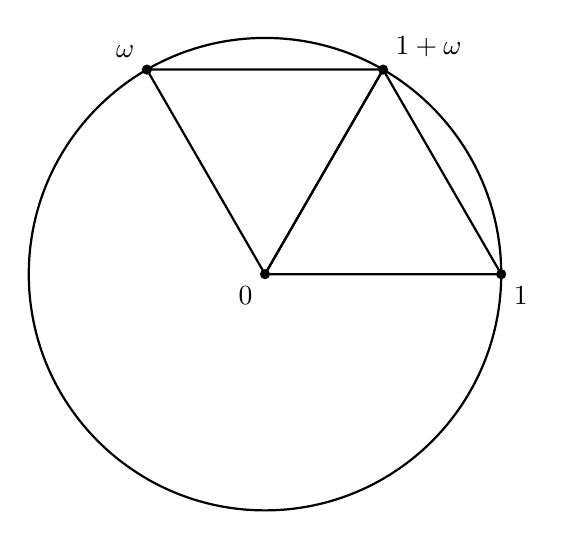
\begin{tikzpicture}[
    point/.style = {circle, fill=black, inner sep=1.3pt},
    scale=3
]

% --- The four points ---
% 0
\coordinate (O) at (0, 0);
% 1
\coordinate (U) at (1, 0);
% omega = (-1 + i sqrt3)/2
\coordinate (W) at (-0.5, 0.8660254);
% 1 + omega
\coordinate (WU) at (0.5, 0.8660254);

% --- Unit circle, centered at 0 ---
\draw[thick] (O) circle (1);

% --- Two equilateral triangles sharing the side O--WU ---
\draw[thick] (O) -- (W) -- (WU) -- cycle;
\draw[thick] (O) -- (U) -- (WU) -- cycle;

% --- Points ---
\foreach \p in {O,U,W,WU} \node[point] at (\p) {};

% --- Labels ---
\node[below left=1pt] at (O) {$0$};
\node[below right=1pt] at (U) {$1$};
\node[above left=1pt] at (W) {$\omega$};
\node[above right=1pt] at (WU) {$1+\omega$};

\end{tikzpicture}
%\caption{Parallelogram.}
%\label{F1}
%\end{figure}
\end{figure}

\begin{prop}\label{Ptri1} 
For all point $P$ in a solid equilateral triangle $\mathcal{T}$ of side length $1$, there is a vertex of $\mathcal{T}$ which is at distance at most $\frac{1}{\sqrt{3}}$ from $P$. 
\end{prop} 

\begin{proof} 
The equilateral triangle $\mathcal{T}$ can be divided into six isometric right triangles with hypothenuse length $\frac{1}{\sqrt{3}}$: see picture below. Since each of these right triangle contains a vertex of $\mathcal{T}$, the conclusion follows from Proposition~\ref{Ptri2} below. 

\begin{figure}[htbp] 
\centering
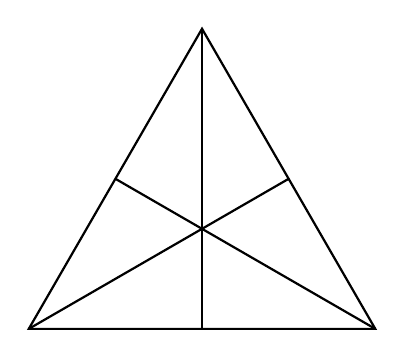
\begin{tikzpicture}[thick, scale=2.2]

% --- Vertices, oriented as (-1, 1, i*sqrt(3)) ---
\coordinate (A) at (-1, 0);
\coordinate (B) at (1, 0);
\coordinate (C) at (0, 1.7320508);

% --- Midpoints of the sides ---
\coordinate (MAB) at ($(A)!0.5!(B)$);
\coordinate (MBC) at ($(B)!0.5!(C)$);
\coordinate (MCA) at ($(C)!0.5!(A)$);

% --- The three sides ---
\draw (A) -- (B) -- (C) -- cycle;

% --- The three medians ---
\draw (A) -- (MBC);
\draw (B) -- (MCA);
\draw (C) -- (MAB);

\end{tikzpicture}
\end{figure}

\end{proof} 

\begin{prop}\label{Ptri2} 
Let $a$ and $b$ be positive real numbers, let $\mathcal{R}$ be the solid rectangle $\{x+iy\in\C\mid 0\le x\le a, 0\le y\le b\}$ contained in the complex plane, and let $z,w$ be in $\mathcal{R}$. Then we have $|z-w|^2\le a^2+b^2$. 
\end{prop} 

\begin{proof}
Setting $z=x+iy, w=u+iv$, we get 
$$
|z-w|^2=(x-u)^2+(y-v)^2\le a^2+b^2.
$$ 
\end{proof} 

Note that Proposition~\ref{Ptri2} holds a fortiori if $\mathcal{R}$ is replaced by a solid right triangle with sides $a,b,\sqrt{a^2+b^2}$ (because $\mathcal{R}$ can be divided into two such right triangles). 

\noindent\textbf{Step 4.} We prove the analogue of Theorem~\ref{T-XIII1}. To do this we first prove the analog of Lemma~\ref{L-XIII}: 

\begin{lem}[In Section~XIII of~\cite{weil1979}]\label{L-XIIIa}
Let $a, b$ be elements of the ring $R$, with $b\ne0$. Then there is a multiple $bq$ of $b$ such that $N(a-bq)<N(b)$. 
\end{lem} 
\begin{proof} 
Let $z$ be any complex number. By Step~3, there is an element $q$ of $R$ such that 
$$
N(z-q)<1.
$$ 
Apply this to $z=\frac{a}{b}$, where $a,b$ are the elements in the lemma. The element $q$ in $R$ defined by the above construction has then the required property. 
\end{proof} 

We now prove the analogue of Theorem~\ref{T-XIII1}, that is, the statement: 

Let $\mathcal{M}$ be a non-empty set of elements in $r$, closed under addition and such that, if $a$ is in $\mathcal{M}$, all multiples of $a$ are in $\mathcal{M}$. Then $\mathcal{M}$ consists of all the multiples of some element $d$ in $R$, uniquely determined up to a unit factor. 

Proof: If $\mathcal{M}=\{0\}$, the theorem is true with $d=0$. If not, take in $\mathcal{M}$ an element $d$ of smallest norm $> 0$. If $a$ is in $\mathcal{M}$, we can apply Lemma~\ref{L-XIIIa} and write $a=dq+r$ with $N(r)<N(d)$. Then $r=a-dq$ is in $\mathcal{M}$, which contradicts the definition of $d$ unless $r=0, a=dq$. As to unicity, if $d'$ has the same property as $d$, then $d$ and $d'$ must be multiples of each other, so that $d'$ is an associate of $d$.

\noindent\textbf{Step 5.} To prove a unique factorization theorem for $R$, we proceed exactly as in the case of Gaussian integers. 

\begin{exer}[Exercise XIII.8 in~\cite{weil1979}]
Use Exercise~\ref{ExXIII7} to show that a rational prime $>3$ can be written as $x^2+xy+y^2$, with integers $x,y$, if and only if it is $\equiv 1\pmod 3$.
\end{exer}

If $x,y$ are rational integers, then 
$$
x^2+xy+y^2=(x-y)^2+3xy\equiv(x-y)^2\pmod{3},
$$ 
so $x^2+xy+y^2$ is congruent to $0$ or $1$ modulo~$3$. Conversely, let $p$ be a rational prime congruent $1$ modulo~$3$. We must show that $p$ can be written as $x^2+xy+y^2$, with ordinary integers $x,y$. Let us compute the Legendre symbol $(\frac{-3}{p})$: 
$$
\left(\frac{-3}{p}\right)=(-1)^{\frac{p-1}{2}}\left(\frac{3}{p}\right)=\left(\frac{p}{3}\right)=1
$$ 
(see Theorem~\ref{Tleg}). So, there is a rational integer $[\sqrt{-3}]$ such that $[\sqrt{-3}]^2 \equiv-3\pmod{p}$. Since $p\ne2$, there is a rational integer $[\frac{1}{2}]$ such that $2\cdot[\frac{1}{2}]\equiv1\pmod{p}$. Defining the rational integer $[\omega]$ by 
$$
[\omega]=(-1+[\sqrt{-3}])\left[\frac{1}{2}\right],
$$ 
we get 
$$
[\omega]^2+[\omega]+1\equiv0\pmod{p}.
$$ 
Note also that the factorization 
$$
[\omega]^2+[\omega]+1=([\omega]-\omega)([\omega]-\omega^2)=([\omega]-\omega)([\omega]+1+\omega)
$$ 
holds in $R$. Since $p$ divides $[\omega]^2+[\omega]+1$, but divides neither $[\omega]-\omega$ nor $[\omega]+1+\omega$, we see that $p$ is not prime in $R$. 

Write $p=q_1\cdots q_k$ with $k\ge1$ and $q_j$ prime in $R$ for all $j$. Since $p$ is not prime in $R$, we have $k\ge2$. The equality $p^2=N(q_1)\cdots N(q_k)$ implies $k=2$ and $p=q_1\overline{q_1}=q_2\overline{q_2}$. Defining the rational integers $x,y$ by $q_1=x-y\omega$, we get $p=N(q_1)=x^2+xy+y^2$. 

\printbibliography

\printindex

\end{document}